% !TEX options = -interaction=batchmode

\documentclass[a4paper]{report}
\usepackage[fontsize=13pt]{scrextend}
%\documentclass[a4paper,draft]{report}
%\pdfcompresslevel=0
%\pdfobjcompresslevel=0
%Compila in modalità batchmode
%Aggiungi i capitoli con \include e quello su cui stai lavorando con \includeonly
%Pare che il todonotes crea seri rallentamenti


% basics
\usepackage[utf8]{inputenc}
\usepackage[T1]{fontenc}
\usepackage{textcomp}
\usepackage[hyphens]{url}
\usepackage[style=alphabetic,maxcitenames=1]{biblatex}
\usepackage[colorlinks=true,linkcolor=cyan,urlcolor=magenta,citecolor=violet]{hyperref}
\usepackage{graphicx}
\usepackage{float}
\usepackage{booktabs}
\usepackage[inline, shortlabels]{enumitem}
\usepackage{emptypage}
\usepackage{subcaption}
\usepackage{multicol}
\usepackage[usenames,dvipsnames]{xcolor}
% quiver style
\usepackage{tikz-cd}
% `calc` is necessary to draw curved arrows.
\usetikzlibrary{calc}
% `pathmorphing` is necessary to draw squiggly arrows.
\usetikzlibrary{decorations.pathmorphing}

% A TikZ style for curved arrows of a fixed height, due to AndréC.
\tikzset{curve/.style={settings={#1},to path={(\tikztostart)
					.. controls ($(\tikztostart)!\pv{pos}!(\tikztotarget)!\pv{height}!270:(\tikztotarget)$)
					and ($(\tikztostart)!1-\pv{pos}!(\tikztotarget)!\pv{height}!270:(\tikztotarget)$)
					.. (\tikztotarget)\tikztonodes}},
	settings/.code={\tikzset{quiver/.cd,#1}
			\def\pv##1{\pgfkeysvalueof{/tikz/quiver/##1}}},
	quiver/.cd,pos/.initial=0.35,height/.initial=0}

% TikZ arrowhead/tail styles.
\tikzset{tail reversed/.code={\pgfsetarrowsstart{tikzcd to}}}
\tikzset{2tail/.code={\pgfsetarrowsstart{Implies[reversed]}}}
\tikzset{2tail reversed/.code={\pgfsetarrowsstart{Implies}}}
% TikZ arrow styles.
\tikzset{no body/.style={/tikz/dash pattern=on 0 off 1mm}}

% useful macro for class
\newcommand{\probability}[2]{\mathbb{\MakeUppercase{P}}_{#1} \left(#2\right)}
\newcommand{\variance}[2]{\mathrm{Var}_{#1} \left[ #2 \right]}
\newcommand{\expectation}[2]{\mathbb{\MakeUppercase{E}}_{#1} \left[#2\right]}
\newcommand{\at}[3]{\left.#1\right\vert_{#2}^{#3}}
\newcommand\quotient[2]{
	\mathchoice
	{% \displaystyle
		\text{\raise1ex\hbox{$#1$}\Big/\lower1ex\hbox{$#2$}}%
	}
	{% \textstyle
		#1\,/\,#2
	}
	{% \scriptstyle
		#1\,/\,#2
	}
	{% \scriptscriptstyle  
		#1\,/\,#2
	}
}
\newcommand{\identity}{\mathrm{id}}
\newcommand{\sinc}{\mathop{\mathrm{sinc}}}
\newcommand{\rect}{\mathop{\mathrm{rect}}}
\newcommand{\tri}{\mathop{\mathrm{tri}}}
\newcommand{\Real}{\mathop{\mathrm{Re}}}

\newcommand{\Homomorphism}{\mathrm{Hom}}
\newcommand{\Morphism}{\mathrm{Mor}}
\newcommand{\Object}{\mathrm{Ob}}

\usepackage{physics}

\DeclareMathOperator{\im}{Im}
\DeclareMathOperator{\sgn}{sgn}
\DeclareMathOperator{\Int}{Int}
\DeclareMathOperator{\diag}{diag}

\let\implies\Rightarrow
\let\impliedby\Leftarrow
\let\iff\Leftrightarrow

\usepackage{stmaryrd} % for \lightning
\newcommand\conta{\scalebox{1.1}{\(\lightning\)}}

\usepackage{bm}
\usepackage{bbm}


% figure support
\usepackage{import}
\usepackage{xifthen}
\pdfminorversion=7
\usepackage{pdfpages}
\usepackage{transparent}
\newcommand{\incfig}[1]{%
	\def\svgwidth{\columnwidth}
	\import{./Figures/}{#1.pdf_tex}
}


%\usepackage{mathptmx}


\usepackage{amsmath, amsfonts, mathtools, amsthm, amssymb}
\usepackage[]{bm}
\usepackage{geometry}
\usepackage{mathrsfs}
\usepackage{cancel}
\usepackage{systeme}
\usepackage[margin=1.5cm,labelfont=bf,font=footnotesize]{caption}
\captionsetup{belowskip=0pt}

\geometry{a4paper,left=2.54cm,right=2.54cm,top=2.54cm,bottom=2.54cm}


% for the big braces
\usepackage{bigdelim}


% correct
\definecolor{correct}{HTML}{009900}
\newcommand\correct[2]{\ensuremath{\:}{\color{red}{#1}}\ensuremath{\to }{\color{correct}{#2}}\ensuremath{\:}}
\newcommand\green[1]{{\color{correct}{#1}}}



% horizontal rule
\newcommand\hr{
	\noindent\rule[0.5ex]{\linewidth}{0.5pt}
}


% hide parts
\newcommand\hide[1]{}



% si unitx
\usepackage{siunitx}
\sisetup{locale = FR}
% \renewcommand\vec[1]{\mathbf{#1}}
\newcommand\mat[1]{\mathbf{#1}}


% tikz
\usepackage{tikz}
\usetikzlibrary{intersections, angles, quotes, positioning}
\usetikzlibrary{arrows.meta}
\usepackage{pgfplots}
\pgfplotsset{compat=1.13}


\tikzset{
	force/.style={thick, {Circle[length=2pt]}-stealth, shorten <=-1pt}
}

% Algorithm Env
\usepackage[linesnumbered,lined,vlined,ruled,commentsnumbered]{algorithm2e}
\SetKwComment{Comment}{// }{}
\SetArgSty{textsl}

% theorems
\makeatother
\usepackage{thmtools}
\usepackage[framemethod=TikZ]{mdframed}

\mdfsetup{skipabove=1em,skipbelow=0em}

\theoremstyle{definition}

\declaretheoremstyle[
	headfont=\bfseries\sffamily\color{YellowGreen!70!black}, bodyfont=\normalfont,
	mdframed={
			linewidth=2pt,
			rightline=false, topline=false, bottomline=false,
			linecolor=YellowGreen, backgroundcolor=YellowGreen!5,
			nobreak=false
		},
]{thmgreenbox}

\declaretheoremstyle[
	headfont=\bfseries\sffamily\color{ForestGreen!70!black}, bodyfont=\normalfont,
	mdframed={
			linewidth=2pt,
			rightline=false, topline=false, bottomline=false,
			linecolor=ForestGreen, backgroundcolor=ForestGreen!8,
			nobreak=false
		},
]{thmgreen2box}

\declaretheoremstyle[
	headfont=\bfseries\sffamily\color{NavyBlue!70!black}, bodyfont=\normalfont,
	mdframed={
			linewidth=2pt,
			rightline=false, topline=false, bottomline=false,
			linecolor=NavyBlue, backgroundcolor=NavyBlue!5,
			nobreak=false
		}
]{thmbluebox}

\declaretheoremstyle[
	headfont=\bfseries\sffamily\color{TealBlue!70!black}, bodyfont=\normalfont,
	mdframed={
			linewidth=2pt,
			rightline=false, topline=false, bottomline=false,
			linecolor=TealBlue,
			nobreak=false
		}
]{thmblueline}

\declaretheoremstyle[
	headfont=\bfseries\sffamily\color{RedOrange!70!black}, bodyfont=\normalfont,
	mdframed={
			linewidth=2pt,
			rightline=false, topline=false, bottomline=false,
			linecolor=RedOrange, backgroundcolor=RedOrange!5,
			nobreak=false
		}
]{thmredbox}

\declaretheoremstyle[
	headfont=\bfseries\sffamily\color{RedOrange!70!black}, bodyfont=\normalfont,
	mdframed={
			linewidth=2pt,
			rightline=false, topline=false, bottomline=false,
			linecolor=RedOrange, backgroundcolor=RedOrange!8,
			nobreak=false
		}
]{thmred2box}

\declaretheoremstyle[
	headfont=\bfseries\sffamily\color{SeaGreen!70!black}, bodyfont=\normalfont,
	mdframed={
			linewidth=2pt,
			rightline=false, topline=false, bottomline=false,
			linecolor=SeaGreen, backgroundcolor=SeaGreen!2,
			nobreak=false
		}
]{thmgreen3box}

\declaretheoremstyle[
	headfont=\bfseries\sffamily\color{WildStrawberry!70!black}, bodyfont=\normalfont,
	numbered=no,
	mdframed={
			linewidth=2pt,
			rightline=false, topline=false, bottomline=false,
			linecolor=WildStrawberry, backgroundcolor=WildStrawberry!5,
			nobreak=false
		},
]{thmpinkbox}

\declaretheoremstyle[
	headfont=\bfseries\sffamily\color{MidnightBlue!70!black}, bodyfont=\normalfont,
	mdframed={
			linewidth=2pt,
			rightline=false, topline=false, bottomline=false,
			linecolor=MidnightBlue, backgroundcolor=MidnightBlue!5,
			nobreak=false
		}
]{thmblue2box}

\declaretheoremstyle[
	headfont=\bfseries\sffamily\color{Gray!70!black}, bodyfont=\normalfont,
	mdframed={
			linewidth=2pt,
			rightline=false, topline=false, bottomline=false,
			linecolor=Gray, backgroundcolor=Gray!5,
			nobreak=false
		}
]{notgraybox}

\declaretheoremstyle[
	headfont=\bfseries\sffamily\color{Gray!70!black}, bodyfont=\normalfont,
	mdframed={
			linewidth=2pt,
			rightline=false, topline=false, bottomline=false,
			linecolor=Gray,
			nobreak=false
		}
]{notgrayline}

% \declaretheoremstyle[
% 	headfont=\bfseries\sffamily\color{RedOrange!70!black}, bodyfont=\normalfont,
% 	numbered=no,
% 	mdframed={
% 			linewidth=2pt,
% 			rightline=false, topline=false, bottomline=false,
% 			linecolor=RedOrange, backgroundcolor=RedOrange!1,
% 		},
% 	qed=\qedsymbol
% ]{thmproofbox}

\declaretheoremstyle[
	headfont=\bfseries\sffamily\color{NavyBlue!70!black}, bodyfont=\normalfont,
	numbered=no,
	mdframed={
			linewidth=2pt,
			rightline=false, topline=false, bottomline=false,
			linecolor=NavyBlue, backgroundcolor=NavyBlue!1,
			nobreak=false
		}
]{thmexplanationbox}

\declaretheoremstyle[
	headfont=\bfseries\sffamily\color{WildStrawberry!70!black}, bodyfont=\normalfont,
	numbered=no,
	mdframed={
			linewidth=2pt,
			rightline=false, topline=false, bottomline=false,
			linecolor=WildStrawberry, backgroundcolor=WildStrawberry!1,
			nobreak=false
		}
]{thmanswerbox}

\declaretheoremstyle[
	headfont=\bfseries\sffamily\color{BrickRed!70!black}, bodyfont=\normalfont,
	numbered=no,
	mdframed={
			linewidth=2pt,
			rightline=false, topline=false, bottomline=false,
			linecolor=BrickRed, backgroundcolor=BrickRed!12,
			nobreak=false
		}
]{thmbrickbox}

\declaretheoremstyle[
	headfont=\bfseries\sffamily\color{OliveGreen!70!black}, bodyfont=\normalfont,
	numbered=no,
	mdframed={
			linewidth=2pt,
			rightline=false, topline=false, bottomline=false,
			linecolor=OliveGreen, backgroundcolor=OliveGreen!1,
			nobreak=false
		}
]{thmolivebox}


\declaretheorem[style=thmolivebox, name=Definition, numberwithin=section]{definition}
\declaretheorem[style=thmgreen2box, name=Definition, numbered=no]{definition*}
\declaretheorem[style=thmredbox, name=Theorem, numberwithin=section]{theorem}
\declaretheorem[style=thmred2box, name=Theorem, numbered=no]{theorem*}
\declaretheorem[style=thmredbox, name=Lemma, numberwithin=section]{lemma}
\declaretheorem[style=thmred2box, name=Lemma, numbered=no]{lemma*}
\declaretheorem[style=thmredbox, name=Proposition, numberwithin=section]{proposition}
\declaretheorem[style=thmred2box, name=Proposition, numbered=no]{proposition*}
\declaretheorem[style=thmredbox, name=Corollary, numberwithin=section]{corollary}
\declaretheorem[style=thmred2box, name=Corollary, numbered=no]{corollary*}
\declaretheorem[style=thmblue2box, name=Claim, numbered=no]{claim}
\declaretheorem[style=thmred2box, name=Details, numbered=no]{details}

% Redefine proof environment to get a full control. 
\makeatletter
\renewenvironment{proof}[1][\proofname]{\par
	\pushQED{\qed}%
	\normalfont \topsep-2\p@\@plus6\p@\relax
	\trivlist
	\item[\hskip\labelsep
	            \color{RedOrange!70!black}\sffamily\bfseries
	            #1\@addpunct{.}]\ignorespaces
	\begin{mdframed}[linewidth=2pt,rightline=false, topline=false, bottomline=false,linecolor=RedOrange, backgroundcolor=RedOrange!1]
		}{%
		\popQED\endtrivlist\@endpefalse
	\end{mdframed}
}
\makeatother

\declaretheorem[style=thmgreenbox, numbered=no, name=Example]{eg}
\declaretheorem[style=thmexplanationbox, numbered=no, name=Proof]{tmpexplanation}
\newenvironment{explanation}[1][]{\vspace{-10pt}\pushQED{\(\circledast\)}\begin{tmpexplanation}}{\null\hfill\popQED\end{tmpexplanation}}

\declaretheorem[style=thmbluebox, numbered=no, name=Remark]{remark}
\declaretheorem[style=thmbrickbox, numbered=no, name=Note]{note}
\declaretheorem[style=thmpinkbox, numbered=no, name=Exercise]{exercise}
\declaretheorem[style=notgrayline, numbered=no, name=As previously seen]{prev}
\declaretheorem[style=thmgreen3box, numbered=no, name=Intuition]{intuition}
\declaretheorem[style=notgraybox, numbered=no, name=Notation]{notation}
\declaretheorem[style=thmpinkbox, numbered=no, name=Problem]{problem}
\declaretheorem[style=thmanswerbox, numbered=no, name=Answer]{tmpanswer}
\newenvironment{answer}[1][]{\vspace{-10pt}\pushQED{\(\circledast\)}\begin{tmpanswer}}{\null\hfill\popQED\end{tmpanswer}}


\usepackage{etoolbox}
\renewcommand{\qed}{\null\hfill\(\blacksquare\)}

\makeatletter

\def\testdateparts#1{\dateparts#1\relax}
\def\dateparts#1 #2 #3 #4 #5\relax{
	\marginpar{\small\textsf{\mbox{#1 #2 #3 #5}}}
}

\def\@lecture{}%
\newcommand{\lecture}[3]{
	\ifthenelse{\isempty{#3}}{%
		\def\@lecture{Lecture #1}%
	}{%
		\def\@lecture{Lecture #1: #3}%
	}%
	\section*{\@lecture}
	\marginpar{\small\textsf{\mbox{#2}}}
}
\usepackage{pgffor}%
\newcommand{\lec}[2]{%
	\foreach \c in {#1,...,#2}{%
			\IfFileExists{Lectures/lec_\c.tex} {%
				\input{Lectures/lec_\c.tex}%
			}{}%
		}%
}

% fancy headers


\usepackage{titleps,kantlipsum}
\newpagestyle{mypage}{%
  \headrule
  \sethead{\thesection\;\sectiontitle}{}{\subsectiontitle}
  \footrule
  \setfoot{\thechapter \; \MakeUppercase{\chaptertitle}}{}{\thepage}
}
\settitlemarks{chapter,section,subsection}
\pagestyle{mypage}

\makeatother

% notes
\usepackage{xargs}                      % Use more than one optional parameter in a new commands

\iffalse
\usepackage[colorinlistoftodos,prependcaption,textsize=scriptsize]{todonotes}


\newcommandx{\Lwtf}[2][1=]{{%
 \let\marginpar\marginnote
 \reversemarginpar
 \renewcommand{\baselinestretch}{0.8}%
 \todo[linecolor=red,backgroundcolor=red!25,bordercolor=red,#1]{#2}}}

\newcommandx{\Lmathwtf}[2][1=]{{%
 \let\marginpar\marginnote
 \reversemarginpar
 \renewcommand{\baselinestretch}{0.8}%
 \text{\todo[fancyline,linecolor=red,backgroundcolor=red!25,bordercolor=red,#1]{#2}}}}

\newcommandx{\Lchange}[2][1=]{{%
 \let\marginpar\marginnote
 \reversemarginpar
 \renewcommand{\baselinestretch}{0.8}%
 \todo[linecolor=blue,backgroundcolor=blue!25,bordercolor=blue,#1]{#2}}}

\newcommandx{\Linfo}[2][1=]{{%
 \let\marginpar\marginnote
 \reversemarginpar
 \renewcommand{\baselinestretch}{0.8}%
 \todo[linecolor=OliveGreen,backgroundcolor=OliveGreen!25,bordercolor=OliveGreen,#1]{#2}}}

\newcommandx{\Lmathinfo}[2][1=]{{%
 \let\marginpar\marginnote
 \reversemarginpar
 \renewcommand{\baselinestretch}{0.8}%
 \text{\todo[fancyline,linecolor=OliveGreen,backgroundcolor=OliveGreen!25,bordercolor=OliveGreen,#1]{#2}}}}


\newcommandx{\Limprovement}[2][1=]{{%
 \let\marginpar\marginnote
 \reversemarginpar
 \renewcommand{\baselinestretch}{0.8}%
 \todo[linecolor=Plum,backgroundcolor=Plum!25,bordercolor=Plum,#1]{#2}}}

 
 
\newcommandx{\wtf}[2][1=]{\todo[linecolor=red,backgroundcolor=red!25,bordercolor=red,#1]{#2}}

\newcommandx{\mathwtf}[2][1=]{\text{\todo[fancyline,linecolor=red,backgroundcolor=red!25,bordercolor=red,#1]{#2}}}

\newcommandx{\change}[2][1=]{\todo[linecolor=blue,backgroundcolor=blue!25,bordercolor=blue,#1]{#2}}

\newcommandx{\info}[2][1=]{\todo[linecolor=OliveGreen,backgroundcolor=OliveGreen!25,bordercolor=OliveGreen,#1]{#2}}

\newcommandx{\mathinfo}[2][1=]{\text{\todo[fancyline,linecolor=OliveGreen,backgroundcolor=OliveGreen!25,bordercolor=OliveGreen,#1]{#2}}}


\newcommandx{\improvement}[2][1=]{\todo[linecolor=Plum,backgroundcolor=Plum!25,bordercolor=Plum,#1]{#2}}

\newcommandx{\thiswillnotshow}[2][1=]{\todo[disable,#1]{#2}}
\fi


\newcommand{\parag}[1]{\paragraph{#1}\mbox{}\\}




\newcommand{\mathexplain}[3][2]{
    \ifthenelse{\equal{\detokenize{#1}}{\detokenize{u}}}{
         \overbracket{#2}^{\mathclap{\textcolor{OliveGreen}{\substack{#3}}}}
         }{}
    \ifthenelse{\equal{\detokenize{#1}}{\detokenize{d}}}{
         \underbracket{#2}_{\mathclap{\textcolor{OliveGreen}{\substack{#3}}}}
         }{}
    \ifthenelse{\equal{\detokenize{#1}}{\detokenize{cu}}}{
         \overbrace{#2}^{\mathclap{\textcolor{OliveGreen}{\substack{#3}}}}
         }{}
    \ifthenelse{\equal{\detokenize{#1}}{\detokenize{cd}}}{
         \underbrace{#2}_{\mathclap{\textcolor{OliveGreen}{\substack{#3}}}}
         }{}
}


\newcommand{\mathwarn}[3][2]{
    \ifthenelse{\equal{\detokenize{#1}}{\detokenize{u}}}{
         \overbracket{#2}^{\mathclap{\textcolor{BrickRed}{\substack{#3}}}}
        }{}
    \ifthenelse{\equal{\detokenize{#1}}{\detokenize{d}}}{
         \underbracket{#2}_{\mathclap{\textcolor{BrickRed}{\substack{#3}}}}
        }{}
    \ifthenelse{\equal{\detokenize{#1}}{\detokenize{cu}}}{
         \overbrace{#2}^{\mathclap{\textcolor{BrickRed}{\substack{#3}}}}
        }{}
    \ifthenelse{\equal{\detokenize{#1}}{\detokenize{cd}}}{
         \underbrace{#2}_{\mathclap{\textcolor{BrickRed}{\substack{#3}}}}
        }{}
}







\usepackage[]{marginnote}
\let\oldmarginpar\marginpar
\renewcommand\marginpar[1]{\-\oldmarginpar[\raggedleft\scriptsize #1]%
{\raggedright\scriptsize #1}}
%\let\marginpar\marginnote

% Fix some stuff
% %http://tex.stackexchange.com/questions/76273/multiple-pdfs-with-page-group-included-in-a-single-page-warning
\pdfsuppresswarningpagegroup=1



\usepackage{import}
\usepackage{xifthen}
\usepackage{pdfpages}
\usepackage{transparent}




% Appendix environment
\usepackage[export]{adjustbox}
\usepackage[many]{tcolorbox}
\usepackage{appendix}

\definecolor{captionbgcolor}{RGB}{103,143,150}

\DeclareCaptionFormat{tcbcaption}{%
  \begin{tcolorbox}[
    colback=captionbgcolor,
    arc=0pt,
    outer arc=0pt,
    boxrule=0pt,
    colupper=white,
    fontupper=\small\sffamily,
    boxsep=0pt
  ]
  #1#2#3
  \end{tcolorbox}%
}
\captionsetup{format=tcbcaption}
\def\chapterautorefname{Section}
\def\sectionautorefname{Section}
\def\appendixautorefname{Appendix}
\renewcommand\appendixname{Appendix}
\renewcommand\appendixtocname{Appendix}
\renewcommand\appendixpagename{Appendix}
% begin appendix autoref patch [\autoref subsections in appendix](https://tex.stackexchange.com/questions/149807/autoref-subsections-in-appendix)
\makeatletter
\patchcmd{\hyper@makecurrent}{%
	\ifx\Hy@param\Hy@chapterstring
		\let\Hy@param\Hy@chapapp
	\fi
}{%
	\iftoggle{inappendix}{%true-branch
		% list the names of all sectioning counters here
		\@checkappendixparam{chapter}%
		\@checkappendixparam{section}%
		\@checkappendixparam{subsection}%
		\@checkappendixparam{subsubsection}%
		\@checkappendixparam{paragraph}%
		\@checkappendixparam{subparagraph}%
	}{}%
}{}{\errmessage{failed to patch}}

\newcommand*{\@checkappendixparam}[1]{%
	\def\@checkappendixparamtmp{#1}%
	\ifx\Hy@param\@checkappendixparamtmp
		\let\Hy@param\Hy@appendixstring
	\fi
}
\makeatletter

\newtoggle{inappendix}
\togglefalse{inappendix}

\apptocmd{\appendix}{\toggletrue{inappendix}}{}{\errmessage{failed to patch}}
\apptocmd{\subappendices}{\toggletrue{inappendix}}{}{\errmessage{failed to patch}}
% end appendix autoref patch

\setcounter{tocdepth}{3}

\newcommand{\ssec}[1]{
	\subsection*{#1}
\subsectionmark{#1}
\addcontentsline{toc}{subsection}{\protect\numberline{} #1}
}
\newcommand{\sssec}[1]{
	\subsubsection*{#1}
\subsubsectionmark{#1}
\addcontentsline{toc}{subsubsection}{\protect\numberline{} #1}
}


\newcommand{\gr}[1]{
	\textcolor{OliveGreen}{#1}}
\newcommand{\red}[1]{
	{\textcolor{BrickRed}}{#1}}







\thispagestyle{empty}
\addbibresource{ref.bib}
\usepackage{adjustbox}
\usepackage{centernot}
\author{Piero Viscone}
\title{Instrumentation for fundamental interactions physics}
\date{}
\begin{document}

\maketitle

\begin{abstract}
	Appunti del corso tenuto dal Prof. Forti (UniPi) sui rivelatori di particelle\\ 
	La quasi totalità del materiale è presa dal libro Particle Detectors (Kolanoski, Wermes) \cite{Kolanoski:2020ksk}
\end{abstract}

\newpage

\tableofcontents
\lec{1}{1}
\newpage
%─────Content────────────────────────────────────────────────────────────────────────────────────────────────────────────────────────────────────────
%Place here the finished chapters
\iffalse

\fi
\chapter{Interazione Radiazione Materia}
Il tempo tipico di decadimento delle particelle dipende dal tipo di interazione:
\begin{itemize}
    \item Forte  < $10^{-22}s$
    \item Debole > $10^{-13}s$
    \item EM $10^{-20}-10^{-14}s$
\end{itemize}
La lunghezza percorsa da una particella prima di decadere è $l=\beta \gamma c \tau_0$ quindi possono essere misurate direttamente protoni, neutroni, elettroni,neutrini (elusivi) e muoni.\\
I $\pi$ e i K possono essere rivelati direttamente ma anche decadere nel rivelatore.
\\
\\
\textbf{Proprietà misurabili} :
\begin{itemize}
    \item \textbf{Momento} : per particelle cariche misurabile tramite il raggio di curvatura in campo magnetico 
    \[ p=q \mathexplain[u]{R}{\text{R ha un segno} 
    \text{ per essere consistente con } 
    \text{la direzione e con la carica}  } B \]

    \item \textbf{Carica} : Direzione della deflessione in campo magnetico
    \item \textbf{Energia}: Misurabile tramite la carica rilasciata o la luce prodotta in un calorimetro
    \item \textbf{Tempo di vita}: Ricostruendo il vertice del decadimento (geometricamente) si può ricavare il tempo in cui è decaduta
    \item \textbf{Velocità}: Tramite TOF, angolo Cherenkov o dal $\frac{dE}{dx}$
    \item \textbf{Massa}: Ottenibile da $m^2=E^2-p^2$ o da $p=m\beta/\sqrt{1-\beta^2} $
\end{itemize}

\section{Interazione di particelle cariche}
I meccanismi di interazione principali per le particelle cariche sono:
\begin{itemize}

    \item \textbf{Eccitazione/Ionizzazione}: Un atomo viene ionizzato rilasciando un $e^-$ poi collezionato per formare un segnale o viene prodotta luce tramite de eccitazione

    \item \textbf{Bremstrahlung}: Particella che viene deflessa dal campo EM nucleare e irraggia (\textit{significativa solo per $e^+$ ed $e^{-}$: particelle leggere})

    \item \textbf{Cherenkov}: Onda d'urto EM prodotta da particelle veloci

    \item \textbf{Radiazione di transizione}: Radiazione emessa quando una particella attraversa un mezzo con indice di rifrazione discontinuo. \marginpar{\gr{Ad esempio nel passaggio tra vuoto e un dielettrico}}\\
    Questo accade perchè il campo elettrico longitudinale subisce un brusco riarrangiamento che, in situazioni di energie molto alte, causa irraggiamento

    L'intensità della radiazione è $\propto \gamma$ quindi può essere usata per misurare velocità

\end{itemize}
\subsection{Particelle massive}
    \subsubsection*{Stopping power}
        Lo stopping power è definito come il $-dE/dx$ per unità di densità del materiale quindi è misurata in MeV cm$^2/g$  ed è espresso in funzione di $\beta \gamma=p/m$.
        \\
        Queste curve, se non normalizzate per la massa della particella, possono essere utili per fare particle identification poichè ogni particella segue una curva a se

        \begin{figure}[H]
            \centering
            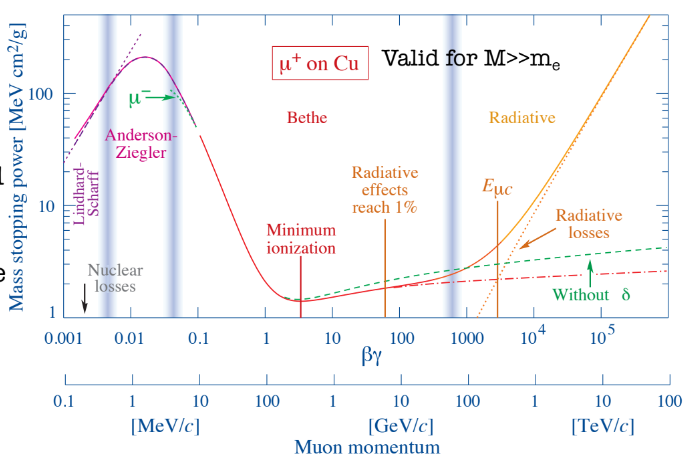
\includegraphics[width=0.8\textwidth,frame]{Chapters/images/Interazione_radiazione_materia/image-20220214171429817.png}
            \caption{Plot dello stopping power per particelle con $M>>m_e$ . Per elettroni e positroni domina Bremstrahlung.\\Possiamo distinguere 3 zone : zona di scattering elastico, di ionizzazione e di Bremstrahlung}
            \label{fig:betheblock}
        \end{figure}
    Analizziamo le diverse regioni della curva:
    \begin{itemize}
        \item Nella zona a più bassa energia (Lindhard-Scharff) si ha un andamento $\propto \beta$ dovuto a scattering elastico su nuclei

        \item La zona di Anderson-Ziegler è ottenuta empiricamente tramite fit su dati sperimentali per mettere un raccordo tra i modelli
        \begin{details}
            In questa zona si ha l' \textbf{effetto Barkas} che consiste in un minore stopping power per particelle negative (dovuto a fattori correttivi di ordine successivo)
        \end{details}


        \item Nella zona di ionizzazione a basse energie si ha un andamento dominato da un fattore cinematico $\sim \beta^{-5/3} \sim \beta^{-2}$

        In questa zona la curva è molto sensibile a variazioni di $\beta$ quindi è possibile ricavare la velocità misurando il $dE/dx$

        \item A circa 3 - 4$\beta \gamma$ si ha il minimo di ionizzazione ed è $\sim 1-2 MeV cm^2/g$

        \item Dopo il minimo di ionizzazione si ha una risalita $\propto ln(\beta \gamma)^2$ dovuta all'estensione relativistica del campo elettrico trasversale ma per grandi $\beta \gamma$ il dielettrico viene polarizzato e si ha una saturazione (\textit{effetto del $\delta$})

        \item Al di sopra dell' \textbf{energia critica} dominano le perdite radiative ovvero la Bremstrahlung e altri processi minori
    \end{itemize}
Concentriamoci un attimo sulle perdite per \textbf{ionizzazione}

\begin{figure}[H]
    \centering
    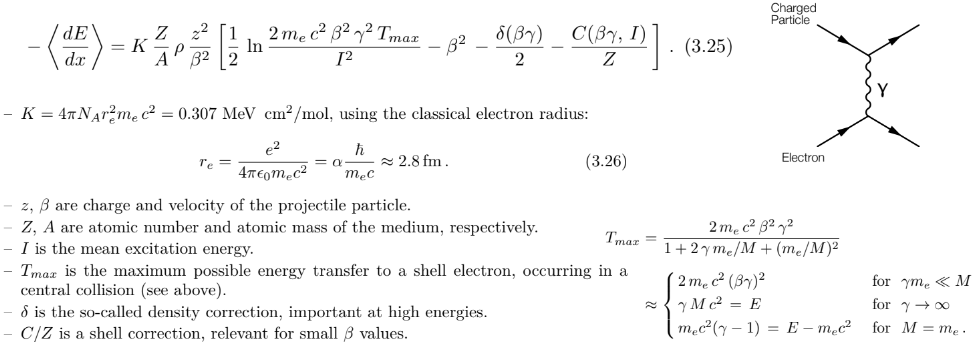
\includegraphics[width=0.95\textwidth,frame]{Chapters/images/Interazione_radiazione_materia/image-20220214173007634.png}
    \captionsetup{width=0.95\linewidth}
    \caption{Bethe-Block: dE/dx dovuta unicamente alla ionizzazione (zona centrale dello stopping power) (e alla radiazione Cherenkov). Non include nè le perdite per bremstrahlung (dominante ad alte energie) nè le perdite per radiazione di transizione}
    \label{fig:betheformula}
\end{figure}





\begin{minipage}{0.48\textwidth}
    \begin{figure}[H]
        \centering
        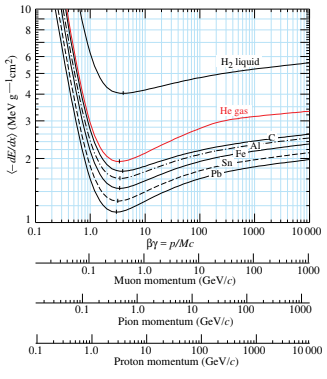
\includegraphics[width=\textwidth,frame]{Chapters/images/Interazione_radiazione_materia/image-20220214175355949.png}
        \captionsetup{width=\textwidth}
        \caption{A: Possiamo vedere come le curve sono essenzialmente indipendenti dal materiale salvo per l'idrogeno. Ricorda che sono normalizzate per la densità}
        \label{fig:}
    \end{figure}
\end{minipage} \hfill
\begin{minipage}{0.48\textwidth}

\begin{figure}[H]
    \centering
    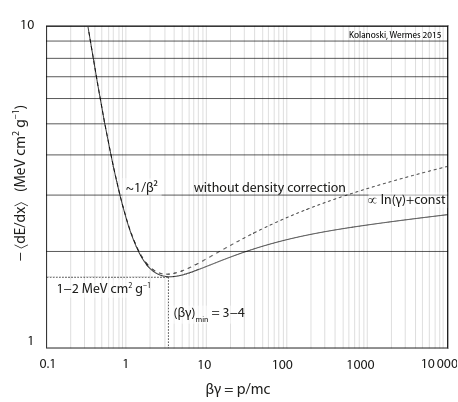
\includegraphics[width=\textwidth,frame]{Chapters/images/Interazione_radiazione_materia/image-20220214175429234.png}
    \captionsetup{width=\textwidth}
    \caption{B: Qui è possibile vedere meglio l'effetto del termine $\delta$ e della dipendenza logaritmica}
    \label{fig:}
\end{figure}

\end{minipage}
Alcune osservazioni sulla Bethe-Block (ionizzazione):
\begin{itemize}
    \item il fattore Z/A, per la formula semiempirica di massa, è più o meno sempre lo stesso $Z/A\sim 0.4$ tranne che per l'idrogeno $H_2$ dove è 1 (poichè non ha neutroni)
    \item A basse energie domina andamento $\sim \beta^{-2}$.
    \item La curva poi risale per 2 motivi:
    \begin{enumerate}
        \item La massima energia trasferibile aumenta con $ \gamma$ (effetto cinematico)
        \item Il campo elettrico trasversale subisce un estensione per effetti relativistici anche se limitato dallo screening degli elettroni atomici che vengono polarizzati (termine $\delta$)
    \end{enumerate}
\end{itemize}

\subsubsection*{Picco di Bragg}

\hspace{-20pt}
\begin{minipage}{0.55\textwidth}
    \begin{figure}[H]
        \centering
        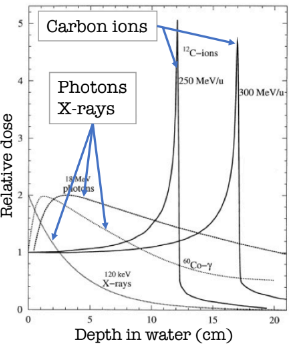
\includegraphics[width=0.75\textwidth,frame]{Chapters/images/Interazione_radiazione_materia/image-20220214183616196.png}
        \captionsetup{width=0.75\textwidth}
        \caption{\\(La dose non è altro che E/M)}
        \label{fig:braggpeak}
    \end{figure}
\end{minipage} \hfill
\begin{minipage}{0.48\textwidth}
    Man mano che la particella perde energia lo stopping power aumenta. E' possibile ricostruire l'energia persa in funzione della penetrazione usando l'andamento $\beta^{-2}$ valido a basse energie

\subsubsection*{Elettroni delta}
Per trasferimenti di energia elevati possono essere strappati elettroni atomici che creano tracce secondarie (sufficientemente lunghe) nella stessa direzione della particella incidente (o comunque a piccoli angoli).
Se il detector non riesce a trattare adeguatamente questi elettroni si può avere un peggioramento della risoluzione spaziale (poichè la carica viene depositata più lontano dal punto di interazione) e fluttuazioni più grandi dello stopping power

\end{minipage}


\subsubsection*{Range}
Il range è la lunghezza percorsa dalla particella nel materiale \[R=\int_{T_0}^0 \left( \frac{dE}{dx} \right)^{-1} dT\] dove $T_0$ è l'energia cinetica iniziale della particella.

\begin{figure}[H]
    \centering
    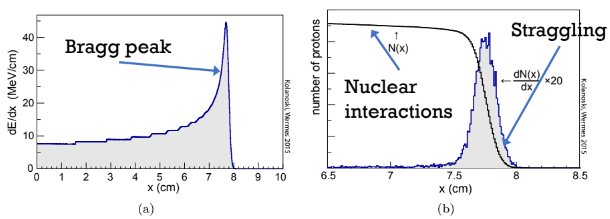
\includegraphics[width=0.95\textwidth,frame]{Chapters/images/Interazione_radiazione_materia/image-20220214185815482.png}
    \captionsetup{width=0.95\linewidth}
    \caption{\textbf{a}: Picco di Bragg \quad \textbf{b}: Straggling }
    \label{fig:straggling}
\end{figure}

\hspace{-20pt}
\begin{minipage}{0.48\textwidth}
    \begin{figure}[H]
        \centering
        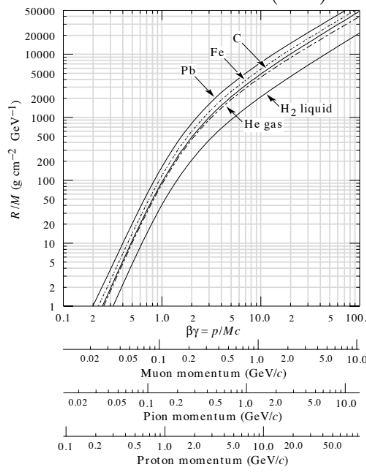
\includegraphics[width=\textwidth,frame]{Chapters/images/Interazione_radiazione_materia/image-20220216172742194.png}
        \captionsetup{width=\textwidth}
        \centering
        \caption{Range normalizzato per la densità del materiale in funzione di $\beta \gamma$.\\
        Plot utile per capire quanto materiale usare in un esperimento}
        \label{fig:}
    \end{figure}
\end{minipage} \hspace{0.5cm}
\begin{minipage}{0.48\textwidth}
    Quando sono coinvolti fenomeni di assorbimento il numero di particelle decresce esponenzialmente (fotoni).
Quando sono coinvolte particelle cariche il numero di particelle rimane pressocchè costante. In figura si vede una lieve diminuzione dovuta a interazioni nucleari.
\\
\\
Si nota anche che il $dN/dx$ non è una delta ma ha una sua larghezza chiamata \textbf{straggling}: questo fenomeno è dovuto alle fluttuazioni statistiche dell'energia rilasciata nel materiale (vedi più avanti)
\\
\\
    Se si esprime l'integrale del range in funzione di $\gamma$ si ha $R=\frac{M}{z^2}f(\gamma_0)$ dove $\gamma_0$ è il $\gamma$ iniziale della particella e $f(\gamma_0)$ è una funzione indipendente dalle proprietà della particella (massa e carica) e dipende solo dal materiale. Quindi il range scala come $M/z^2$ (riferite alla particella)

\end{minipage}
\subsection{Particelle poco massive ($e^{+} ; e^{-})$}
Per le particelle cariche poco massive (elettroni e positroni) vale quanto detto sopra ma sono presenti dei fenomeni aggiuntivi:
\begin{itemize}


    \item La \textbf{bremstrahlug}
    \item Gli elettroni incidenti scatterano con elettroni atomici: Sono particelle identiche, interviene il principio di pauli
    \item Per positroni va considerata l'annichilazione con gli elettroni atomici

    Generalmente, oltre a prendere in considerazione la bremstrahlung, vanno considerati 2 regimi di energia:
    \begin{itemize}
        \item Quando i livelli energetici degli elettroni atomici NON possono essere trascurati si fa la media come nel caso di particelle massive
        \item Quando si hanno grandi trasferimenti di energia vengono considerati gli scattering Moller ($e^- e^- \to e^- e^-$) e Bhabha ($e^+ e^- \to e^+ e^-$)
    \end{itemize}


\end{itemize}

\begin{figure}[H]
    \centering
    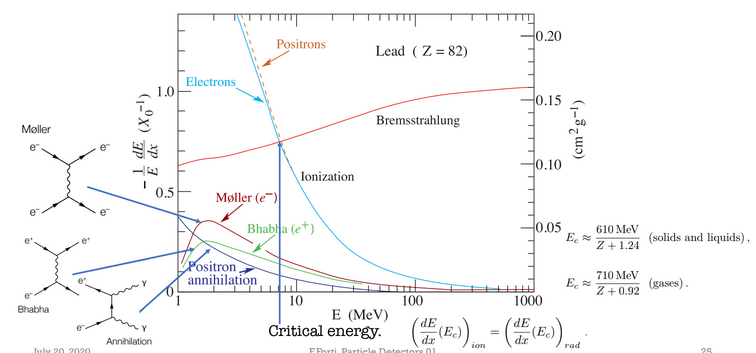
\includegraphics[width=0.95\textwidth,frame]{Chapters/images/Interazione_radiazione_materia/image-20220217021527324.png}
    \captionsetup{width=0.95\linewidth}
    \caption{Per particelle leggere il dE/dx è molto diverso in quanto la bremmstrahlung diventa dominante già sotto il GeV, nel piombo già a 7MeV \\ Anche qui si nota l'effetto per il quale la particella con carica negativa a basse energie perde un po' meno energia}
    \label{fig:electronloss}
\end{figure}
\subsubsection*{Bremstrahlung e lunghezza di radiazione}
Consiste nell'irragiamento dovuto alla deflessione dell'elettrone causata dal campo elettrico nucleare (scattering Rutherford con il nucleo)
\newline
L'energia emessa per una carica accelerata, sia nel limite classico che quantistico, è $dE/dt \propto \frac{1}{m^2}$

\begin{note}
    Ad altissime energie (es. LHC) la bremmstrahlung diventa rilevante anche per muoni e pioni
\end{note}

\[-\frac{dE}{dX} \Bigr|_\text{Brem} =\frac{E}{X_{0}} \quad \implies \quad  E(x) = E_{0} e^{\frac{-x}{X_{0} }} \]

\[\rho X_{0} =\frac{716.408 \: A \: \text{mol/g}}{Z(Z+1)\ln \frac{287}{\sqrt{Z} }} \frac{\text{g} }{\text{cm}^{2}  }
    \]
 $X_0$ è chiamata \textbf{lunghezza di radiazione} e corrisponde alla lunghezza dopo il quale l'energia di un \textbf{elettrone} è ridotta di un fattore $1/e$ (per bremmstrahlung)

\begin{note}
    La lunghezza di radiazione è definita solo per elettroni in quanto per altre particelle molto energetiche come muoni le fluttuazioni di energia sono molto grandi e spesso sono associate a sciamature quindi parlare di perdita di energia come un processo uniforme e continuo è insensato
\end{note}
\begin{remark}

    Si noti la dipendenza (molto approssimativa a causa del log.) $-\frac{dE}{dx} \sim \propto E Z^2$

\end{remark}
Tipicamente la Bremmstrahlung viene emessa in avanti o comunque a piccoli angoli $\theta \sim1/\gamma=m/E$

\begin{figure}[H]
    \centering
    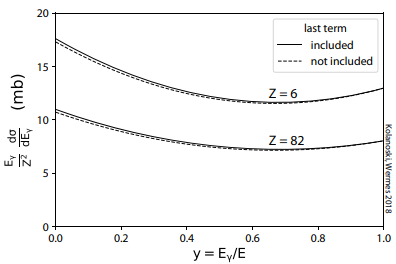
\includegraphics[height=4.5cm,frame]{Chapters/images/Interazione_radiazione_materia/image-20220220135143452.png}
    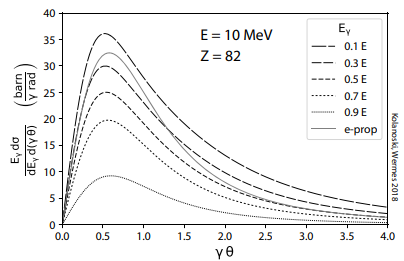
\includegraphics[height=4.5cm,frame]{Chapters/images/Interazione_radiazione_materia/image-20220220135223580.png}
    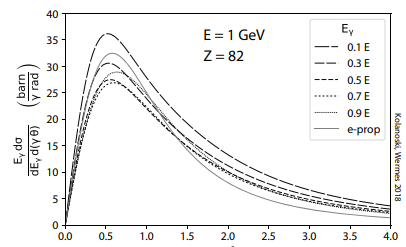
\includegraphics[height=4.5cm,frame]{Chapters/images/Interazione_radiazione_materia/image-20220220135322598.png}
    \captionsetup{width=0.9\linewidth}
    \caption{\textbf{A} : Spettro della Bremmstrahlung per C e Pb normalizzata per fattore $E_\gamma/Z^2$ \\ \textbf{B} ,\textbf{C} : distribuzione angolare della Bremmstrahlung a diverse energie}
    \label{fig:}
\end{figure}
Inoltre quando avviene Bremmstrahlung dobbiamo considerare vari possibili fenomeni:
\begin{itemize}
    \item Correzioni di \textbf{Coulomb}:  Correzione dovuta all'interferenza della funzione d'onda della particella con il campo coulombiano

\item \textbf{Suppressione dielettrica}: Fotoni emessi a piccole energie vengono assorbiti nel materiali a causa della polarizzabilità del materiale causando una perdita di coerenza e un cutoff infrarosso nello spettro del fotone

\item La \textbf{bremmstrahlung}  può avvenire anche con il campo elettrico degli elettroni atomici (basta sostituzione $Z^2 \to Z(Z+1)$)

\item Effetto \textbf{LPM} : Ad altissime energie (sopra il TeV) la Bremmstrahlung (e la produzione di coppie) è soppressa .
\end{itemize}
  Ad alte energie per energie perse piccole l'interazione avviene su lunghe distanze. Se questa distanza è maggiore del cammino libero medio (distanza media tra 2 eventi successivi) la prima emissione interferisce con la seconda introducendo causando una soppressione nello spettro dei fotoni
\subsection{Fluttuazioni statistiche}
La Bethe block determina solo il $dE/dx$ medio ma in realtà l'energia rilasciata è soggetta a fluttuazioni.

L'energia persa $\Delta E$ in un tratto $\Delta x$ è la somma di tutti i processi di eccitazione/ionizzazione lungo il tratto percorso $\Delta E= \sum^N_{n=1} \delta E_n$.\\
Ci sono 2 contributi statistici:
\begin{itemize}
    \item Uno dovuto al numero di ionizzazioni/eccitazioni (conteggio)
    \item Uno dovuto all'energia emessa dal processo

    Queste fluttuazioni possono causare una serie di problemi

    \item \textbf{Incertezza sul momento}:Per ricostruire il momento di una particella solitamente si usa la Bethe Block per capire quanta energia ha perso nel detector ma le fluttuazioni statistiche introducono un'incertezza sull'energia persa e quindi anche sul momento
    \item \textbf{Incertezze nel PID} poichè la particle identification si fa soprattutto tramite le misure del $dE/dx$ è introdotta un incertezza anche su questo
    \item \textbf{Incertezze nel tracking}: I tracker sono solitamente sottili quindi soffrono delle fluttuazioni poissoniane. Inoltre la risoluzione spaziale è ulteriormente ridotta dagli elettroni delta che possono anche causare ionizzazioni secontarie

\end{itemize}

\subsubsection*{Fluttuazioni del numero di processi}
E' una fluttuazione di tipo \textbf{Poissoniano}, rilevante soprattutto in detector sottili (molto usati nel tracking) e l'incertezza relativa è
\[\frac{\sigma(\Delta E)}{\Delta E}\sim\frac{1}{\sqrt{N}}\]

\begin{remark}

    In caso di rivelatore spesso 1cm di Argon questa incertezza è del 10%
\\
    I rivelatori a semiconduttore invece necessitano energie molto più basse per produrre una coppia elettrone lacuna quindi vengono creati molti più elettroni e l'incertezza è molto ridotta rispetto i rilevatori a gas

\end{remark}

\subsubsection*{Fluttuazioni dell'energia rilasciata}
Dalla distribuzione angolare degli elettroni emessi nel processo di ionizzazione si trova che tra un valore $\delta E_{min}$ (dato dall'energia di ionizzazione dell'atome) e un valore $\delta E_{max}$ (dato da constraint cinematici) la distribuzione di $\delta E$ ha un andamento $\sim 1/(\delta E)^2$ .
\\
Il massimo della distribuzione si ha intorno a $\delta E_{min}$ ma ricordiamo che per energie più alte si presenta il problema degli elettroni delta

\subsubsection*{Distribuzione di Landau-Vavilov}

Generalmente le fluttuazioni nell'energia rilasciata portano a una distibuzione asimmetrica composta da una parte gaussiana (dovuta a piccole perdite di energia) e una lunga coda (per grandi perdite di energia)

\begin{note}
    A causa dell'asimmetria della distribuzione il valore più probabile di energia rilasciata NON è quello che vediamo nella Bethe Block (che è la media) che è un po' più alto della moda della distribuzione
\end{note}
Il primo a trovare una distribuzione fu \textbf{Landau} sotto le seguenti ipotesi:
\begin{itemize}
    \item $lim_{k \to0} T_{max}= +\infty$
    \item Gli elettroni sono trattati come quasi liberi, sono trascurati gli effetti di legame per bassi valori dell'energia trasferita
    \item La perdita di energia della particella nel mezzo può essere trascurata
\end{itemize}

\[
\begin{gathered}
    f_L(\lambda)=\frac{1}{\pi}\int_0^\infty e^{-t ln (t)-\lambda t }\sin (\pi t) dt
\\
\;\;\lambda=\frac{\Delta E -\Delta E_w}{\xi} \;\;
\\
\;\;\Delta E_w=\text{Massimo della distr.}
\end{gathered}\]
La forma della distribuzione dipende dal parametro $k=\xi/T_{max}$ dove $T_{max}$ è l'energia cinetica massima cedibile a un elettrone e $\xi \propto \rho\frac{Z}{A}\frac{z^2}{\beta^2} \Delta x$  è il fattore moltiplicativo presente nella bethe block quindi, almeno nell'andamento \[\mathbf{\xi \simeq dE/dx}\]
\begin{itemize}
    \item \textbf{k grande implica distribuzione simmetrica (Gaussiana)}
\item \textbf{k piccolo implica distribuzione asimmetrica}

\end{itemize}
La distribuzione di landau è un'ottima \textbf{approssimazione per piccoli valori di k}

\hspace{-20pt}
\begin{minipage}{0.48\textwidth}
    \begin{figure}[H]
        \centering
        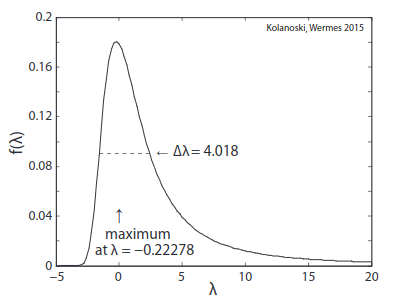
\includegraphics[width=\textwidth,frame]{Chapters/images/Interazione_radiazione_materia/image-20220216191943021.png}
        \captionsetup{width=\textwidth}
        \caption{Distribuzione di Landau. Il $\Delta \lambda$ è la larghezza a metà altezza}
        \label{fig:landau}
    \end{figure}
\end{minipage} \hspace{0.2cm}
\begin{minipage}{0.5\textwidth}
\begin{remark}
    La landau può essere approssiamata dalla distribuzione di Moyal $f(\lambda)=\frac{1}{\sqrt{2\pi}}e^{-0.5(\lambda+e^{-\lambda})}$
In questo caso però $\lambda$ perde il senso fisico che ha nella landau per questo è preferibile usare la Landau
\end{remark}
\textbf{Vavilov}  generalizzò la distribuzione anche per grandi valori di k ma comunque mantenendo l'assunzione che gli effetti di legame siano trascurabili per piccoli davoli di energia trasferita.
Questa distribuzione ha 2 parametri aggiuntivi rispetto alla distribuzione di Landau
\end{minipage}
\begin{details}
    Senza entrare nel dettaglio la Vavilov è definita tramite una trasformata di Laplace
\end{details}
\subsubsection*{Soppressione delle fluttuazioni}

La fluttuazioni possono essere ridotte se la moda della distribuzione può essere usata come uno stimatore dell'energia persa al posto della media poichè la moda gode di uno stimatore migliore (La distribuzione ha una coda molto lunga quindi la media aritmetica potrebbe avere una varianza molto grande rispetto alla moda soprattutto ad alte energie)

\hspace{-20pt}
\begin{minipage}{0.52\textwidth}
    \begin{figure}[H]
        \centering
        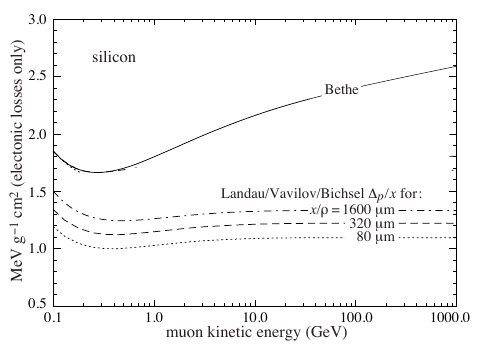
\includegraphics[width=\textwidth,frame]{Chapters/images/Interazione_radiazione_materia/image-20220217014236788.png}
        \captionsetup{width=\textwidth}
        \caption{Le curve tratteggiate sono relative alla moda invece che alla media. Si nota che ad alte energie la media sale molto di più rispetto alla moda}
        \label{fig:landaumode}
    \end{figure}
\end{minipage} \hfill
\begin{minipage}{0.48\textwidth}
    Altri metrodi per eliminare incertezze sono:
\begin{itemize}
    \item Escludere gli elettroni deltra dalle misurse (Possibile in cloud/bubble chamber e in layer indipendenti molto sottili di un detector)
    \item Usare una media troncata scartando i valori più alti e più bassi (Stima più robusta)
    \item Ricostruire l'energia persa dalla particella durante il suo percorso e non solo alla fine (Utile nella misura del momento.)
\end{itemize}


\end{minipage}
\subsection{Multiplo Scattering}
In un materiale possono avvenire scattering multipli. Questi causano un'incertezza nella direzione della particella.
La distribuzione angolare dell'angolo di scattering medio può essere ben approssimata  con una gaussiana (per limite centrale)
\begin{remark}
    per un numero finito e fissato di scattering c'è distribuzione di Moliere che però predice probabilità più alte per grandi angoli come Rutherford
\end{remark}
\begin{figure}[H]
    \centering
    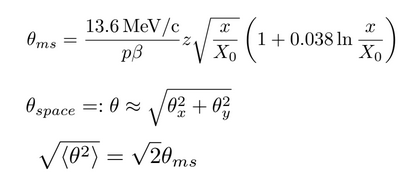
\includegraphics[width=0.8\textwidth,frame]{Chapters/images/Interazione_radiazione_materia/image-20220217025524958.png}
    \captionsetup{width=0.8\linewidth}
    \caption{Deviazione standard dell'angolo di scattering nell'approssimazione gaussiana a piccoli angoli (valida al di sopra dei 20MeV)}
    \label{multiplescattering}
\end{figure}
\begin{figure}[H]
    \centering
    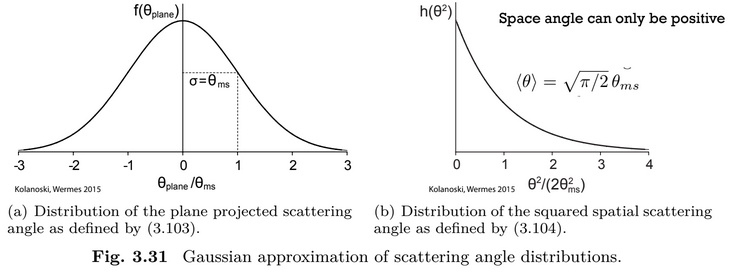
\includegraphics[width=0.8\textwidth,frame]{Chapters/images/Interazione_radiazione_materia/image-20220217030024845.png}
    \captionsetup{width=0.8\linewidth}
    \caption{NB: l'angolo ha un segno.\\Se si considera il valore assoluto dell'angolo la distribuzione cambia}
    \label{fig:mmscatteringradius}
\end{figure}
\subsection{Radiazione Cherenkov}
La radiazione Cherenkov avviene quando una particella carica attraversa un mezzo a una velocità maggiore della velocità della luce nello stesso mezzo causando un'onda d'urto luminosa.
\\
Quello che viene prodotto è un cono luminoso con una apertura angolare di $\cos(\theta_c)=\frac{1}{n\beta}$ , questo significa che la luce cherenkov può essere usata per trovare $\beta$ (e se si è misurato in qualche altro modo il momento anche la massa) o come threshold in quanto viene emessa solo per $\beta>1/n$
\\
L'energia persa per radiazione cherenkov è solitamente molto bassa e trascurabile (Comunque inclusa nella bethe bloch nelle perdite radiative)
\subsection{Misture}
Soprattutto nei detector gassosi possono essere presenti più materiali insieme
\begin{figure}[H]
    \centering
    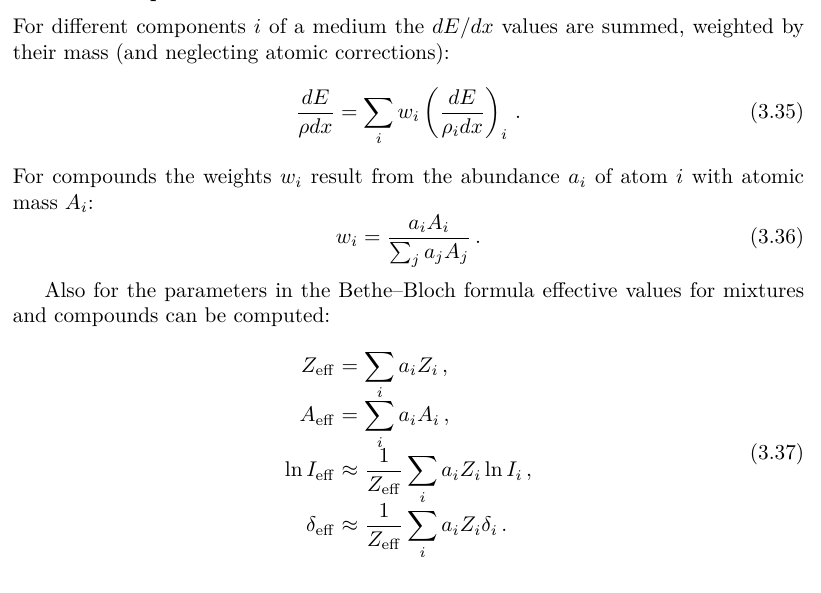
\includegraphics[width=0.95\textwidth,frame]{Chapters/images/Interazione_radiazione_materia/image-20220217042603821.png}
    \captionsetup{width=0.95\linewidth}
    \label{fig:misture}
\end{figure}
Per la lunghezza di radiazione invece \[\frac{1}{\rho X_0}|_{\text{eff.}}=\sum_i \frac{1}{\rho_i X_{0_i}}\]

\section{Interazione di fotoni}
\begin{figure}[H]
    \centering
    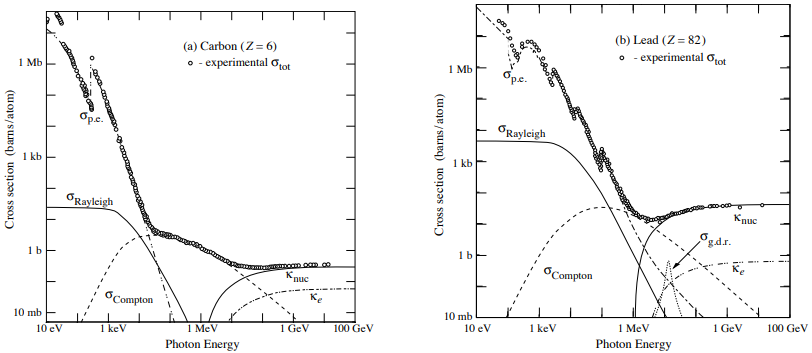
\includegraphics[width=0.95\textwidth,frame]{Chapters/images/Interazione_radiazione_materia/image-20220220114414907.png}
    \captionsetup{width=0.95\linewidth}
    \caption{\\ $k_e$: Produzione di coppie nel campo degli elettroni\\$k_n$: Produzione di coppie nel campo dei nuclei\\$\sigma_{g.d.r.}$: Interazione fotonucleare\\ \\Si noti come per materiali leggeri l'effetto compton è dominante per un range molto più ampio di energia e comunque sempre dominante intorno a 1MeV}
    \label{fig:}
\end{figure}
Le interazioni principali dei fotoni con la materia sono:
\begin{itemize}
    \item \textbf{Scattering Thomson}: Scattering del $\gamma$ a bassa energia su un elettrone libero. L'onda EM accelera (fa oscillare) la carica che emette radiazione di dipolo (a livello classico la frequenza dell'onda deve essere inferiore al periodo di rotazione classico dell'elettrone intorno al nucleo).
    \\
     Sugli $e^-$ corrisponde al limite di bassa energia del compton.
     A differenza del raylight si ha su corpi non polarizzabili (cariche libere)

    \item \textbf{Scattering Rayleight}: Scattering elastico coerente sugli atomi o molecole. Se la frequenza dell'onda è bassa questa polarizza la materia creando dei dipoli che irraggiano.
    Dipende principalmente dalla grandezza del corpo su cui scattera, dalla sua polarizzabilità e dalla sua frequenza di risonanza

    \item \textbf{Effetto fotoelettrico}: Il fotone trasferisce tutta l'energia all'atomo che emette un elettrone

    \item \textbf{Effetto compton}: Scattering elastico $\gamma \; e^- \to \gamma \; e^-$

    \item \textbf{Produzione di coppie}: Nel campo elettrico del nucleo

    \item \textbf{Interazioni fotonucleari}: Mai dominanti e presenti solo in range determinati di energia nel gamma.
    Consistono nell'eccitazione di un nucleone che decadendo emette un protone, un neutrone o un alpha (rilevante nelle supernove).
    Per determinati materiali questo processo può causare fissione
\end{itemize}
I fotoni vengono asssorbiti o scatterati con una probabilità proporzionale alla lunghezza percorsa nel mezzo.
\\
\\
Data n la densità del mezzo  e N il numero di fotoni, si ha

\[
\begin{gathered}
\text{Coefficiente di assorbimento : }\mu=-\frac{1}{N}\frac{dN}{dx}=n \sigma
\\
\text{Cammino libero medio  :  } \lambda=\frac{1}{\mu}=\frac{1}{n\sigma}
\end{gathered}
\]
\begin{remark}
    Si noti che anche in questo caso queste grandezze vengono normalizzate per la densità del materiale
\end{remark}
Quindi il numero di fotoni in funzione della penetrazione sarà
\[ N(x)=N_0e^{-\mu x}=N_0e^{-\frac{x}{\lambda}}=N_0e^{-n\sigma x} \]

\begin{figure}[H]
    \centering
    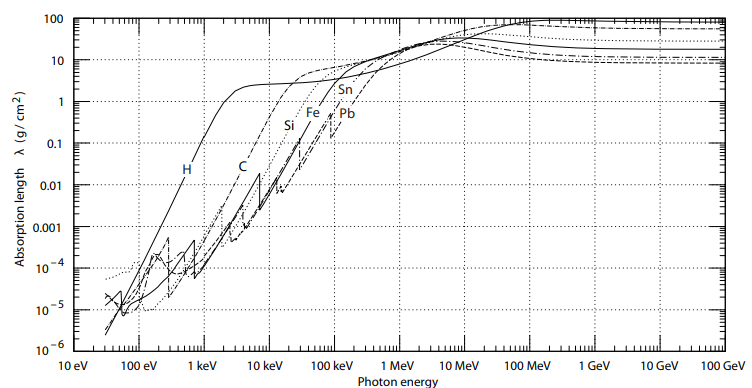
\includegraphics[width=0.95\textwidth,frame]{Chapters/images/Interazione_radiazione_materia/image-20220220113210434.png}
    \captionsetup{width=0.95\linewidth}
    \caption{Cammino libero medio (normalizzato per la densità) in funzione dell'energia del fotone in diversi materiali}
    \label{fig:freemeanpath}
\end{figure}
\subsection{Effetto fotoelettrico}
Processo $\gamma \; \text{atom} \to \text{atom}^+ \; e^-$ dominante nella regione bassa del KeV.
\\
Poichè accada il fotone deve avere un'energia superiore all'energia di legame dell'elettrone, l'energia che avanza va in energia cinetica dell'elettrone. (il rinculo del nucleo è trascurabile)
\\
La dipendenza della sezione d'urto fotoelettrica è
\[\sigma_{p.e.} \propto \frac{Z^5}{E_\gamma}\]
Quindi è \textbf{fortemente dipendente dal materiale usato}
\begin{details}
    In realtà per basse energie la legge di potenza Z varia tra 4 e 5 poichè diventa rilevante la struttura elettronica dell'atomo
\end{details}
\begin{figure}[H]
    \centering
    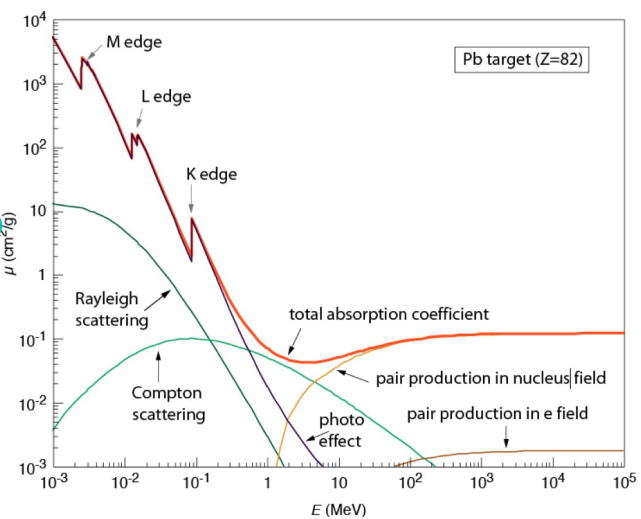
\includegraphics[width=0.8\textwidth,frame]{Chapters/images/Interazione_radiazione_materia/image-20220220120913778.png}
    \captionsetup{width=0.8\linewidth}
    \caption{Inoltre crescendo con l'energia la sezione d'urto (e l'energia cinetica dell' elettrone rilasciato) presenta bruschi picchi dovuti alla possibilità di accedere agli orbitali atomici più interni}
    \label{fig:gammacrossec}
\end{figure}
\subsubsection*{Emissione secondaria}
Il "buco" lasciato dall'effetto fotoelettrico in uno shell interno viene riempito da un elettrone di uno shell superiore. Questo processo causa l'emissione di altra energia o tramite un fotone o tramite un \textbf{elettrone Auger} ovveroun elettrone che scende ad occupare un orbitale più interno causa, tramite l'interazione coulombiana (scambio di un fotone), l'emissione di un elettrone negli orbitali più esterni.

\begin{details}
L'energia rilasciato da questo processo (sia tramite fotone che emissione auger) è discreta quindi causa linee molto riconoscibili negli spettri.
\\
Inoltre la probabilità di emissione di un fotone secondario aumenta con Z mentre quella di un elettrone auger diminuisce con Z
\end{details}
\vspace{5pt}
Le emissioni secondarie in generale possono presentare "Artifici" chiamati picchi di uscita.
Ad esempio se dopo un'interazione fotoelettrica viene emesso un fotone secondario che esce dal detector l'energia del fotone sarà persa quindi si osserverà un secondo picco con energia pari a quella del fotopicco meno l'energia di transizione tra gli orbitali che hanno generato il fotone secondario. (Per gli auger invece solitamente vengono assorbiti dal detector e contribuiscono al fotopicco)

\subsection{Effetto Compton}
Avviene quando l'energia del fotone incidente è molto maggiore di quella di legame dell'elettrone, in questo libite l'elettrone si può considerare libero.
\\
Può capitare che l'elettrone rimanga legato e tutto l'atomo subisca un rinculo. Questo accade con sempre più probabilità con il calare dell'energia infatti nel limite di bassa energia si ottiene lo scattering Thomson.
\\
Il compton è dominante intorno a 1MeV e la regione in cui domina è tanto più ampia quanto piccolo Z (questo perchè il fotoelettrico va come $Z^5/E_\gamma$ quindi per alti Z la regione in cui domina è maggiore)
\begin{remark}
    Proprio perchè intorno a 1MeV si ha prevalentemente solo Compton per queste energie è veramente difficile schermare i fotoni a causa della totale assenza di fenomeni di assorbimenti
\end{remark}
La sezione d'urto compton su singolo elettrone è indipendente da Z MA al crescere dell'energia sempre più elettroni atomici possono essere considerati quasi liberi quindi la \textbf{sezione d'urto compton su un atomo} è
\[\sigma_C^{\text{atom}}=Z\sigma_C\]

\vspace{-10pt}
\hspace{-20pt}
\begin{minipage}{0.48\textwidth}
    \begin{figure}[H]
        \centering
        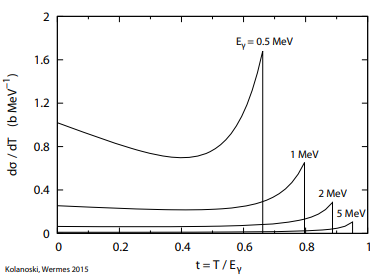
\includegraphics[width=\textwidth,frame]{Chapters/images/Interazione_radiazione_materia/image-20220220124719776.png}
        \captionsetup{width=\textwidth}
        \caption{Il limite massimo dell'energia cinetica dell'elettrone è chiamato compton edge ed è sempre inferiore al fotopicco.}
        \label{fig:comptonedge}
    \end{figure}
\end{minipage} \hfill
\begin{minipage}{0.48\textwidth}
    \vspace{5pt}
    \subsubsection*{Spalla Compton}
    \raggedright
    Il massimo dell'energia cinetica dell'elettrone si ha per il backscattering del fotone. Questo effetto, nello spettro dell'energia cinetica dell'elettrone, è chiamato \textbf{compton edge}
\vspace{-5pt}
\subsubsection*{Compton inverso}
Ci si riferisce allo stesso processo del compton ma nel caso in cui si abbia uno scattering tra fotoni di bassa energia e elettroni di alta energia.
\\
Questo processo produce fotoni di alta energia ed è rilevante nella produzione di gamma rays astrofisici nell'energia del TeV

\end{minipage}
\subsection{Produzione di coppie}
La threshold di produzione di coppie è poco sopra al doppio della massa dell'elettrone $1.02MeV$ (a causa del rinculo del nucleo trascurabile).
\\
La produzione di coppie \textbf{è  strettamente legata con la bremmstrahlung}

\hspace{-20pt}
\begin{minipage}{0.48\textwidth}
    \begin{figure}[H]
        \centering
        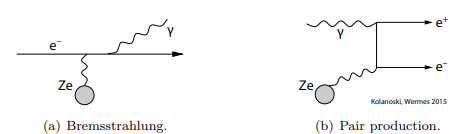
\includegraphics[width=\textwidth,frame]{Chapters/images/Interazione_radiazione_materia/image-20220220131152626.png}
        \captionsetup{width=\textwidth}
        \caption{L'unica differenza è nel riordinamento del grafo}
        \label{fig:brempair}
    \end{figure}
\end{minipage} \hfill
\begin{minipage}{0.48\textwidth}
Quindi anche gli elementi di matrice sono correlati, almeno all'ordine leading e anche tutte le soppressioni dovute allo schermaggio degli elettroni atomici sono uguali a quelle resentui nel caso della bremmstrahlung.
\end{minipage}
\vspace{10pt}
\\


\vspace{-10pt}
\hspace{-20pt}
\begin{minipage}{0.48\textwidth}
    \begin{figure}[H]
        \centering
        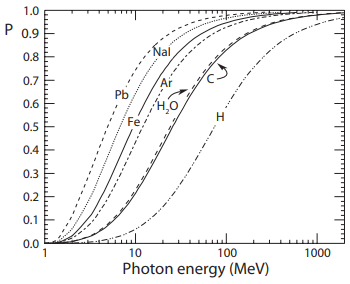
\includegraphics[width=\textwidth,frame]{Chapters/images/Interazione_radiazione_materia/image-20220220132317352.png}
        \captionsetup{width=\textwidth}
        \caption{Probilità della produzione di coppie in diversi materiali.\\A queste energie il resto delle interazioni è praticamente completamente compton}
        \label{fig:pairmaterials}
    \end{figure}
\end{minipage} \hfill
\begin{minipage}{0.48\textwidth}
    Facendo i calcoli si può scrivere la \textbf{lunghezza di assorbimento} per la produzione di coppie in funzione della lunghezza di radiazione per bremmstrahlung
\[\lambda_{\text{pair}}=\frac{1}{n_{\text{atoms}}\sigma_\text{pair}}=\frac{9}{7}X_0\]
Mentre la sezione d'urto è $\sigma_{pair_{nucl}}\propto Z^2$ a causa della somma dei contributi di tutti i nucleoni.\\
    \textbf{Questo  vale solo per la produzione di coppie  in campo nucleare} in quanto il corpo su cui avviene la produzione deve assorbire il rinculo e, mentre il  rinculo del nucleo è trascurabile, quello degli elettroni no quindi ha una threshold più alta.
\end{minipage}
\subsection*{Recap: interazione dei fotoni}



\begin{minipage}{0.48\textwidth}
    \begin{figure}[H]
        \centering
        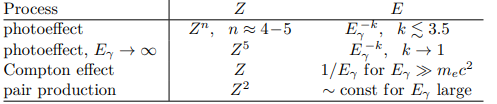
\includegraphics[width=1\textwidth,frame]{Chapters/images/Interazione_radiazione_materia/tabella.png}
        \captionsetup{width=1\textwidth}
        \caption{Processo dominante in funzione di Z del materiale e dell'energia del fotone}
        \label{fig:recapgamma}
    \end{figure}
\end{minipage} \hfill
\begin{minipage}{0.48\textwidth}
    \begin{figure}[H]
        \centering
        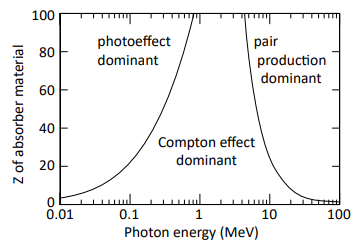
\includegraphics[width=1\textwidth,frame]{Chapters/images/Interazione_radiazione_materia/image-20220220132720070.png}
        \captionsetup{width=1\linewidth}
        \label{fig:}
    \end{figure}


\end{minipage}
\section{Interazioni Adroniche}
Per gli adroni, oltre agli effetti di ionizzazione già discussi, sono presenti anche interazioni adroniche (tipicamente forti) che possono essere di svariato tipo (elastico, inelastico, di cattura, di fissione, di trasferimento,etc.) ma tipicamente questi processi generano particelle cariche
\\
Come per i fotoni viene introdotto il concetto di lunghezza di assorbimento che dipende solo dai processi inelastici
\\
Per adroni di altissima energia la lunghezza di assorbimento è circa costante $\lambda_a=\frac{1}{n\sigma_{\text{inel}}} \propto A^{-2/3}$ (A massa atomica)
\\
Per alti Z tipicamente la lunghezza di assorbimento è molto più grande della lunghezza di radiazione (questo perchè le interazioni forti hanno range di interazione corto e quindi bassa probabilità), per questo motivo i calorimetri adronici devono essere molto più grandi di quelli elettromagnetici.
\\
E' possibile definire anche una lunghezza di interazione dove si considerano sia i processi elastici che inelastici ma solitamente i processi adronici elastici non trasferiscono molta energia quindi sono irrilevanti e anche le deflessioni causate sono trascurabili.
\\
Per i neutroni le interazioni adroniche sono le uniche possibili quindi diventano molto penetranti
\section{Interazione di neutrini}
I neutrini interagiscono molto debolmente, sono poco massivi e anche neutri
\\
Le tipiche reazioni cercate sono:
$\nu+n \to (e,\mu,\tau) +p$ o corrispondente con le antiparticelle
\\
Per 1km di acqua la probabilità di interazione per un neutrino da 200 GeV è $\sim 6 \cdot 10^{-15}$ quindi sono necessari detector enormi con tonnellate di acqua/ghiaccio o scintillatore o grandi sandwitch di convertitore/detector.


\chapter{Formazione del segnale}

Tipicamente i detector sfruttano le cariche generate dalle particelle che ionizzano la materia e sfruttano campi elettrici e magnetici per spostarle.
\\
Nel detector possiamo distinguere 2 tipi di movimenti:
\begin{itemize}
    \item \textbf{Disordinati}: con una distribuzione di velocità (Maxwell-Boltzmann nel limite classico. Nei semi conduttori può diventare importante l'effetto quantistico) data dall'energia termica che causa una dispersione della carica. Il campo elettrico può cambiare questa distribuzione
    \item \textbf{Moto di drift}: causato dalla presenza di campi elettrici e magnetici
\end{itemize}
La \textbf{velocità di drift} è data dall'equilibri dell'accelerazione della carica e le collisioni con gli altri atomi.
Solitamente $|v_d|\ll \left<v\right>$ dove $\left<v\right>$ è la media della velocità termica

\section{Equazione del trasporto}
L'\textbf{equazione di boltzmann} descrive l'evoluzione di posizione e velocità di una carica in un mezzo in funzione delle forze esterne. 
\\ 
\\ 
Consideriamo una nuvola di cariche in un mezzo con una distribuzione nello spazio delle fasi f (dp è un elemento infinitesimo dello spazio delle fasi)

\begin{figure}[H]
    \centering
    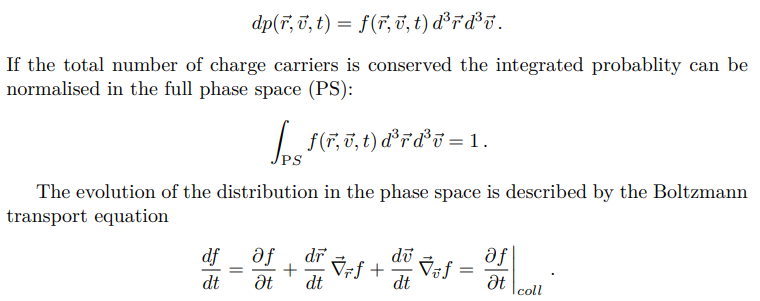
\includegraphics[width=0.8\textwidth,frame]{Chapters/images/Interazione_radiazione_materia/image-20220222095029391.png}
    \captionsetup{width=0.8\linewidth}
    \caption{Equazione del trasporto di Boltzmann}
    \label{fig:boltzmann}
\end{figure}
\begin{remark}[Commenti]
\hfill
\begin{itemize}
    \item $\partial_t f=0$ nel caso non ci sia dipendenza esplicita della densità dello sp. delle fasi dal tempo. 
  Quindi \textit{è nullo nel caso stazionario}

\item 2° termine descrive evoluzione nella posizione (diffusione)

\item 3° termine descrive evoluzione nella velocità

\item $\partial_tf|_\text{coll}$ è detto integrale di collisione (infatti eq. Boltzmann è un'equazione integro-differenziale). In questo termine entrano tutte le possibili sezioni d'urto a cui le cariche sono soggette
\end{itemize}


\end{remark}

\begin{note}[Integrale di collisione]
    \[\at{\frac{\partial f}{\partial t}}{coll}{}=\int W(\vec{v}_1,\vec{v} _{2} ;\vec{v} _{3}, \vec{v}) \{ f(\vec{r} ,\vec{v} _{1} ,t)f(\vec{r} , \vec{v} _{2} t)-f(\vec{r} ,\vec{v} _{3},t) f(\vec{r} ,\vec{v} ,t)\} d \vec{v} _{1} d \vec{v} _{2} d \vec{v} _{3}   \]


\begin{figure}[H]
    \centering
    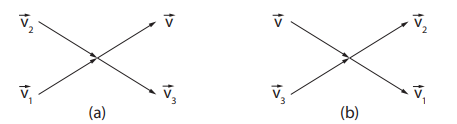
\includegraphics[width=0.8\textwidth,frame]{Chapters/images/Interazione_radiazione_materia/image-20220222100641937.png}
\end{figure}
    \hspace{-15pt}
    \begin{minipage}{0.48\textwidth}
        \begin{figure}[H]
            \centering

            \captionsetup{width=\textwidth}
            \caption{\\
            A: Il termine positivo è dato dall'aumento di densità causato all'aumento della velocità a causa di una collisione entrante che fa accelerare la particella \\
            B: Il termine negativo rappresenta una  diminuzione della densità causata dalla collisione della particella con altri atomi che ne causa una perdità di energia}
            \label{fig:}
        \end{figure}
    \end{minipage} \hspace{20pt}
    \begin{minipage}{0.4\textwidth}
    
        Integrale di collisione nel caso di scattering elastico $1+2\to3+4$.\\
         E' la probabilità che la particella 1 e 2 che si incontrano al tempo t nel punto r scatterino in una seconda coppia con velocità v e $v_3$ e viceversa (W è simmetrica per scambio delle coppie)
    
    \end{minipage}
\end{note}

\subsubsection*{Approssimazioni}
Alcune approssimazioni utili che rendono l'equazione analiticamente risolvibile sono:
\begin{itemize}
    \item \textbf{Equilibrio (Maxwell-boltzmann)}: Caso in cui non ci sono forze e f(r,v,t)=f(v). In questo caso l'integrale di collisione è nullo.

$$
f_0(\vec{v})=C \exp(-Av^2)
$$

\item \textbf{Approssimazione di rilassamento}: Assumiamo che dopo un'interazione il sistema impieghi un \textit{tempo di rilassamento} $\tau$ per tornare all'equilibrio. 
  Sotto questa assunzione vale $\partial_tf|_\text{collision}=-\frac{f-f_0}{\tau}$ dove $f_0$ è la soluzione nel caso di equilibtio. 
  La soluzione sarà:
  $$
  f(t)=f_0+(f-f_0)e^{-\frac{t}{\tau}}
  $$
  Questa approssimazione è \textit{molto utile nei detector} che sono sistemi in qui l'equilibrio è ripristinato dopo un tempo caratteristico

  \item \textbf{Campo elettrico costante}: In questa approssimazione possiamo considerare la presenza di un campo elettrico costante: 
    \begin{itemize}
        \item Il 1° termine è nullo, stabilità implica indipendenza temporale

    \item Il 2° termine è nullo
    \item Il 3° termine è dato da $\frac{dv}{dt}=\frac{qE}{m}$
    \end{itemize}
    

    Un'altra approssimazione che si può fare è $\nabla_v f \sim \nabla_vf_0$

    Se esprimiamo tutto in funzione dell'energia cinetica T otteniamo
    $$
    f= f_0-eQ\tau v_3\partial_Tf_0
    $$
    Ovviamoente la distribuzione è anisotropa e preferisce la direzione del campo E

\end{itemize}

\subsection{Velocità di Drift}
La \textbf{velocità di drift} è la velocità media (vettoriale) delle cariche
$$
\vec{v_D}=\int \vec{v} f(\vec{v})d^3\vec{v}
$$
Questa velocità è non nulla solo se f presenta una asimmetria nello spazio degli impulsi.
Conviene rappresentare questa asimmetria in termini di distribuzioni angolari e quindi esprimendo le velocità in coordinate sferiche.
\\ 
Esprimendo l'integrale in funzione dell'energia cinetica otteniamo 
\[
\begin{gathered}
        \vec{v_d}=\frac{2qE}{3m}<\tau>=\mu E
    \\ 
    \text{Mobilità: }\mu=\frac{2q}{3m} \left<\tau \right>\; :
    \\ 
    \text{Cammino libero medio: }\lambda=\tau v=\frac{1}{n\sigma}  
\end{gathered}  
\]
\begin{remark}[Misture]\hfill \\ 
    Per le misture vale $\frac{1}{\mu}=\sum_i \frac{f_i}{\mu_i}$ dove $f_i$ sono le abbondanze. 
Questa legge vacilla quando iniziano a esserci importanti scambi di carica tra gli ioni e le molecole del gas con diversa mobilità
\end{remark}
Il tempo medio $\tau$ che intercorre tra 2 successive collisioni è dato dalle sezioni d'urto in gioco ed è esprimile in funzione del cammino libero medio.

\begin{note}
    $\tau$ non è il tempo di rilassamento come definito prima ma è il tempo di collision. Ad ogni collisione le velocità sono in media distribuite isotropicamente e l'energia guadagnata dalla particella è dispersa, quindi il sistema torna all'equilibrio
\end{note}
La mobilità è fortemente dipendente dal campo E in quanto lo sono anche tutte le sezioni d'urto coinvolte nelle collisioni. Questo causa fenomeni di saturazione (o addirittura di diminuzione nei gas) della velocità di drift per campi elettrici molto alti.

\begin{remark}[Presenza di campo magnetico]
    \hfill
    \\
    \hspace{-20pt}
\begin{minipage}{0.48\textwidth}
    \begin{figure}[H]
        \centering
        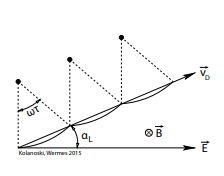
\includegraphics[width=\textwidth,frame]{Chapters/images/Interazione_radiazione_materia/image-20220222150553652.png}
        \captionsetup{width=\textwidth}
        \caption{Angolo di Lorentz}
        \label{fig:lorentzangle}
    \end{figure}
\end{minipage} \hspace{10pt}
\begin{minipage}{0.48\textwidth}
    Nel caso sia presente anche un campo B non si hanno cambiamenti nella velocità di drift e si ha una riduzione della diffusione: le cariche percorrono archi di curve.\\ 
    \\
    L'angolo formato dalla traccia con il campo elettrico sarà $\tan(\alpha_L)=\frac{v^B_x}{v^E_z}=w\tau$ dove z è la direzione del campo elettrico e $\omega=qB/m$ è la frequenza di ciclotrone.
$\alpha_L$ è detto \textbf{Angolo di Lorentz}

\end{minipage}
\end{remark}

\subsection{Diffusione}
Dall'equazione di continuità e di diffusione della corrente (legge di Fick) si ottiene l' equazione di diffusione
\[ \mathexplain[cu]{\frac{\partial \rho }{\partial t} +\vec{\nabla} \cdot \vec{j} _{D} =0}{\text{continuity}} \quad \quad ; \quad \quad \mathexplain[cu]{\vec{j} _{D}=-D \vec{\nabla} \rho  }{\text{Fick's law on} \\ \text{diffusion current} } \quad \quad ; \quad \quad \mathexplain[cu]{\frac{\partial \rho }{\partial t} -D \nabla^2  \rho }{\text{ Diffusion equation}} 
 \]
 dove D è detto \textbf{coefficiente di diffusione } e vale $D=\frac{\left<\lambda v\right>}{3}$
\\ 
 Dopo aver percorso un distanza x la dispersione della carica avrà una larghezza $\sigma_x=\sqrt{2Dt}=\sqrt{\frac{2\epsilon_kx}{qE}}$ dove $\epsilon_k$ è l'energia termica (che all'equilibrio termico è $\epsilon_k=kT$)
 \\ 
 Per la relazione di \textit{Nernst-Townsend-Einstein} vale $\epsilon_k=\frac{qD}{\mu} \geq kT$ (questa relazione non vale in presenza di campi esterni e l'uguaglianza vale all'equilibrio termico)
\begin{note}
    L'argon ha una grande dispersione in quanto non c'è nulla che limiti i moti vibrazionali e rotazionali delle molecole. Quello che si fa di solito è usare l'argon in misture con altri gas che sono vicini al limite termico come metano,isobutano, co2, etc.
\\ 
    (L'argon va usato sia poichè è inerte sia perchè essendo un nucleo più pesante Z=16 favorisce la ionizzazione)
\end{note}
\newpage

\section{Moto delle cariche nei gas}
\subsection*{Velocità di Drift}
\begin{itemize}
    \item \textbf{Ioni}: A causa della loro massa hanno una velocità di drift molto minore della loro velocità termica quindi si possono considerare all'equilibrio.
  La mobilità è praticamente indipendente dal campo elettrico in quanto la sezione d'urto dei processi coinvolti è abbastanza costante con l'energia quindi vale $\epsilon_k=kT$ e $n=p/kT\implies \lambda=kT/(p\sigma)$.

  Il moto degli ioni ha un ruolo importante nella formazione del segnale all'anodo (dove avviene la moltiplicazione degli elettroni)

\item \textbf{Elettroni}: Le sezioni d'urto che coinvolgono gli elettroni sono fortemente energy dependent a causa della scarsa massa degli elettroni. 
  Inoltre sono presenti anche processi inelastici che causano delle perdite di carica (fortemente energy dependent, dipendono dalle linee di assorbimento del materiale).
  \begin{itemize}
    \item Le molecole pesanti tendono a spostare la distribuzione id energia a valori più bassi (a causa dei vari moti vibrazionali e rotazionali della molecola).

    \item Per campi elettrici molto alti la velocità di drift (e quindi la mobilità) tende a diminuire
  \end{itemize}
\end{itemize}



  \begin{figure}[H]
    \centering
    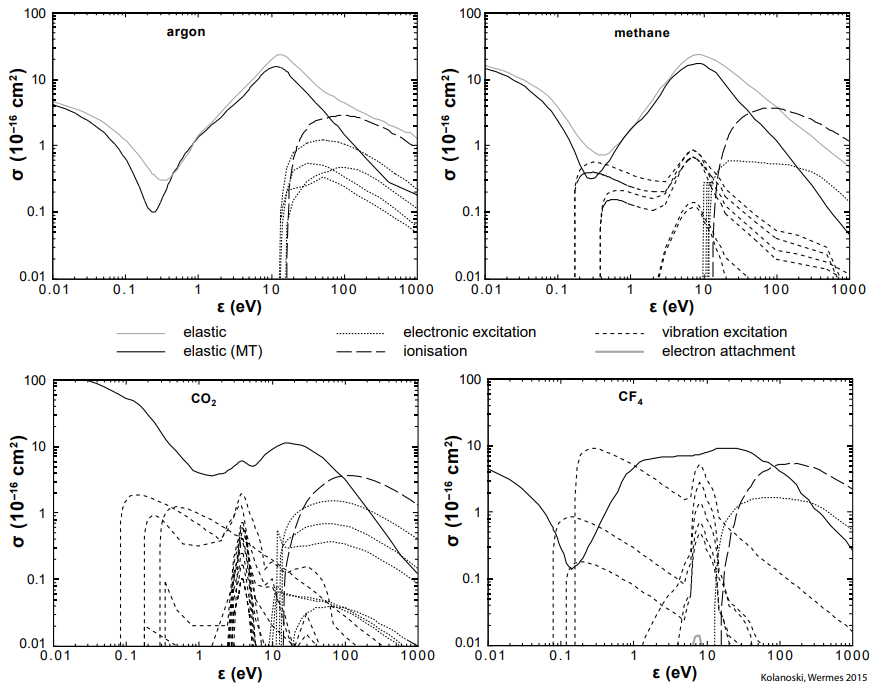
\includegraphics[width=0.95\textwidth,frame]{Chapters/images/Interazione_radiazione_materia/image-20220222172045918.png}

  \end{figure}

  \begin{figure}[H]
    \centering
    \captionsetup{width=0.95\linewidth}
    \caption{Sezioni d'urto in funzione dell'energia.\\ Si noti che per molecole semplici si ha per lo più solo scattering elastico.\\ Nelle regioni di scattering elastico la mobilità cresce molto all'aumentare dell'energia}
    \label{fig:gascross}
  \end{figure}




 \vspace{-20pt}
  \begin{remark}[Mistura argon metano]  \hfill \\ 
\hspace{-50pt}
  \begin{minipage}{0.32\textwidth}
    \begin{figure}[H]
        \centering
        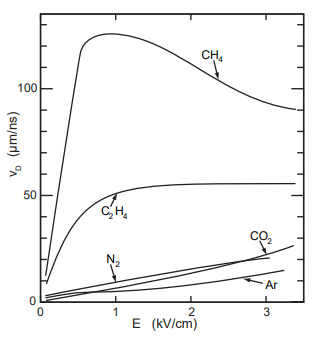
\includegraphics[height=4.8cm,frame]{Chapters/images/Interazione_radiazione_materia/image-20220222172819847.png}
    \end{figure}
  \end{minipage} \hspace{-10pt}
  \begin{minipage}{0.64\textwidth}
  \begin{figure}[H]
    \centering
    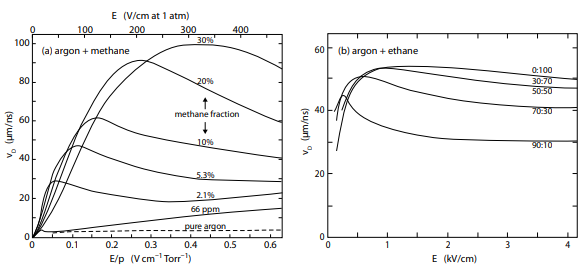
\includegraphics[height=4.8cm,frame]{Chapters/images/Interazione_radiazione_materia/image-20220222172607946.png}
  \end{figure}

  \end{minipage}
\begin{figure}[H]
    \captionsetup{width=\textwidth}
    \caption{Andamento della velocità di drift in funzione del campo elettrico per diversi materiali.}
    Aggiungere metano all' argon causa una diminuzione nella distribuzione di energia degli elettroni quindi le sezioni d'urto diminuiscono e la velocità di drift aumenta.\\ 
    Infatti tipicamente viene aggiunto metano all'argon.
\end{figure}

  \end{remark}
\subsection*{Diffusione}
Nei gas si è spesso al di fuori del limite termico e la dispersione è un problema serio che va moderato

\hspace{-25pt}
\begin{minipage}{0.7\textwidth}
    \begin{figure}[H]
        \centering
        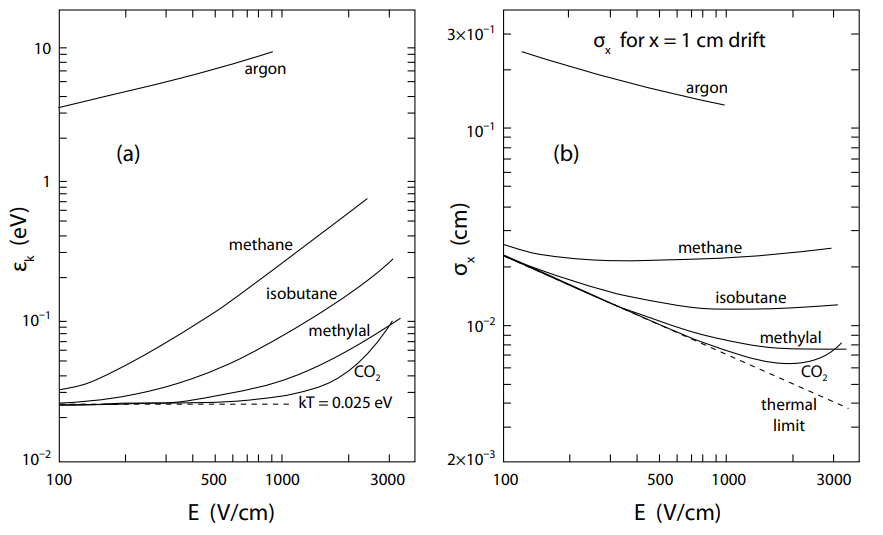
\includegraphics[width=\textwidth,frame]{Chapters/images/Interazione_radiazione_materia/image-20220222180147403.png}
    \end{figure}
\end{minipage}
\begin{minipage}{0.35\textwidth}
\begin{figure}[H]
    \centering
    \captionsetup{width=\textwidth}
    \caption{A: Energia caratteristica per diversi gas in funzione del campo elettrico. (Il limite termico si ha per campo elettrico nullo)
    \\ B: Dispersione per centimetro percorso in vari gas.\\ Si noti come una carica dell'argon, dopo aver percorso 1cm, ha già 1mm di dispersione circa}
\end{figure}
\end{minipage}

\hspace{-25pt}
\begin{minipage}{0.35\textwidth}
    \begin{figure}[H]
        \centering
        \captionsetup{width=\textwidth}
        \caption{La dispersione non è isotropa e spesso bisogna tenere conto delle differenze tra quelle longitudinali e quelle trasversali (quindi abbiamo due coefficienti di dispersione $D_T$ e $D_L$)\\ Addirittura in presenza di campo B l'anisotropia è così forte che D va scritto in forma tensoriale}
    \end{figure}
\end{minipage} \hfill
\begin{minipage}{0.7\textwidth}

    \begin{figure}[H]
        \centering
        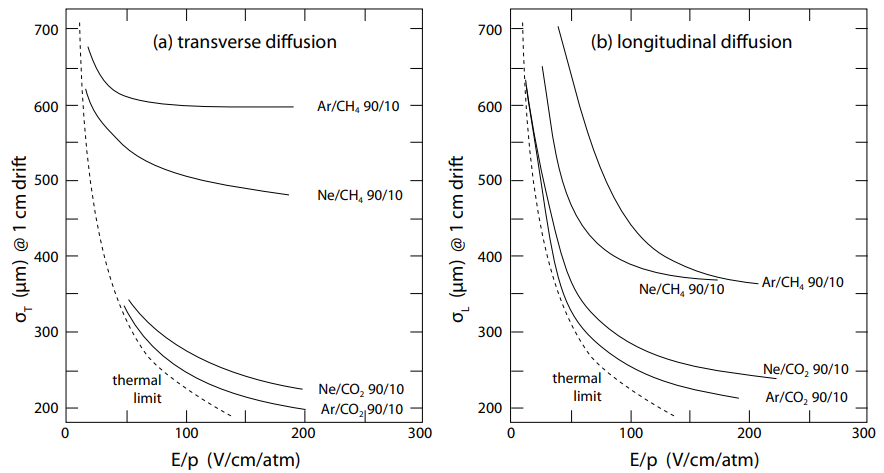
\includegraphics[width=\textwidth,frame]{Chapters/images/Interazione_radiazione_materia/image-20220222180339979.png}
        \captionsetup{width=\textwidth}
    \end{figure}
\end{minipage}

\newpage
\section{Moto delle cariche nei semiconduttori}
La massa (effettiva) delle lacune non è perfettamente definita ma p comparabile a quella degli elettroni quindi il comportamento delle cariche positive è totalmente diverso da quello degli ioni nei gas.

\subsection*{Velocità di Drift}
Lo scattering nel reticolo, prevalentemente dovuto alle impurità, è molto diverso reispetto a quello nei gas (quindi cambia l'integrale di collisione) e le perdite di energia in fononi  può essere molto rilevante

\hspace{-30pt}
\begin{minipage}{0.55\textwidth}
    \vspace{-40pt}
    \begin{figure}[H]
        \centering
        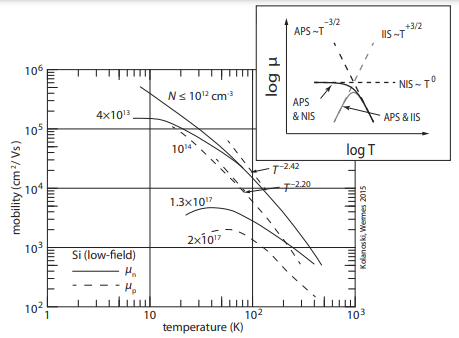
\includegraphics[width=\textwidth,frame]{Chapters/images/Interazione_radiazione_materia/image-20220223184712151.png}
        \captionsetup{width=\textwidth}
        \caption{Mobilità in funzione della temperatura per diverse densità di doping. \\ Nel caso di temperature moltobasse la mobilità è molto alta, per questo motivo si costruiscono rivelatori criogenici.\\ Nota che la curva APS significa "acustic phono scattering"}
        \label{fig:}
    \end{figure}
\end{minipage} \hspace{5pt}
\begin{minipage}{0.5\textwidth}

    Anche qui è presente un effetto di \textbf{saturazione} : la velocità di drift cresce con il campo elettrico fino ad arrivare a una saturazione e, in alcuni casi, anche a una diminuzione per campi elettrici molto alti (a causa di scattering inelastici con fononi di più alta energia).\\ 
    Una buona descrizione della velocità di drift può essere data da:
    $$
    v_d=\mu(E) E =\frac{\mu_0 E}{[1+(\frac{\mu_0 E}{v_{\text{sat}}})^\beta]^{^{1/\beta}}}
    $$
    dove $\mu_0$ è la mobilità a basso campo, $v_{\text{sat}}$ è la velocità di saturazione e $\beta$ è un parametro empirico (genericamente diverso per elettroni e lacune) con un valore tra 1 e 2.\\
    Ad esempio per il \textbf{silicio} (fattore 3): \[\begin{gathered}
        \mu_n=1450 cm^2/(Vs) \; \\  \; \mu_p=500 cm^2/(Vs)
    \end{gathered}\] 
\\ \\ 
\end{minipage}
\vspace{-40pt}\par\noindent\hspace*{0pt}\ignorespaces
Nei gas la mobilità era dell'ordine di $10 cm^2/\text{Vs} $ per gli ioni e $10^4 cm^2/\text{Vs} $ per gli $e^{-}$ 

\hspace{-20pt} 
\begin{minipage}{0.55\textwidth}
    \vspace{-5pt}
    \begin{figure}[H]
        \centering
        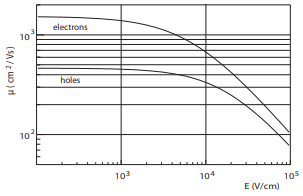
\includegraphics[width=\textwidth,frame]{Chapters/images/Interazione_radiazione_materia/image-20220223185948941.png}

        \label{fig:mobilitae}
    \end{figure}
\end{minipage} \hspace{5pt}
\begin{minipage}{0.48\textwidth}
\begin{figure}[H]
    \centering
    \captionsetup{width=\textwidth}
    \vspace{-10pt}
    \caption{Mobilità di elettroni e cariche in funzione del campo elettrico nel silicio a temperatura ambiente}
\end{figure}
\vspace{-30pt}
    \begin{note}Nei semiconduttori è possibile arrivare a campi elettrici molto maggiori visto che le differenze di potenziale sono applicate su scale molto più piccole (microscopiche), quindi non c'è bisogno di arrivare a voltaggi esagerati come nei rivelatori a gas
    
    \end{note}

\end{minipage}

\begin{figure}[H]
    \centering
    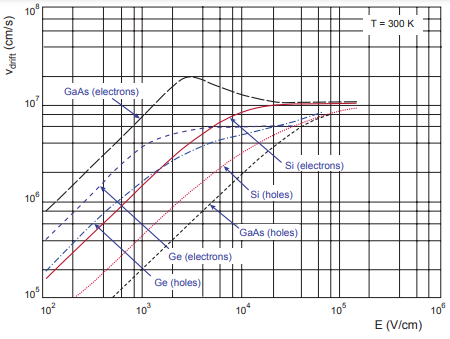
\includegraphics[width=0.9\textwidth,frame]{Chapters/images/Interazione_radiazione_materia/image-20220223190024373.png}
    \captionsetup{width=0.9\textwidth}
    \caption{Velocità di drift in funzione del campo elettrico. Si noti che prima della saturazione la velocità di drift è proporzionale al campo (slope $\simeq1$)}
    \label{fig:driftvel}
\end{figure}
\subsection*{Diffusione}
Come nel caso degli ioni nei gas, nei semiconduttori si è vicini al limite termico quindi vale approssimativamente $\epsilon_k=qD/\mu=kT$ (ovviamente si ha un D e un $\mu$ diverso per elettroni e lacune)

\section{Formazione del segnale (Schokley-Ramo)}
Quando la carica si avvicina a un elettrodo su esso viene indotta una carica del segno opposto . Mettendo l'elettrodo a possiamo far fluire una corrente
\begin{note}non è la collezione della carica a formare il segnale ma la carica indotta. Quando la caricha prodotta dalla ionizzazione viene collezionata dall'elettrodo  il segnale cessa di esistere

\end{note}

\subsection{Wighting field}
Consideriamo una carica q che si muove in un sistema di 2 elettrodi
\begin{figure}[H]
    \centering
    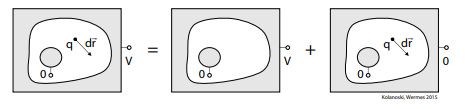
\includegraphics[width=0.7\textwidth,frame]{Chapters/images/Interazione_radiazione_materia/image-20220223201749719.png}
    \captionsetup{width=0.7\textwidth}
\end{figure}
La differenza di potenziale tra i due elettrodi induce una carica Q e -Q su di essi. Data la capacità del sistema si ha $Q=CV$.
\begin{itemize}
    \item Una carica in moto tra gli elettrodi induce una carica addizionale e il campo elettrico fa un lavoro $ dW_q=q \vec{E_0} d\vec{r} $

\begin{remark}\hfill \\ 
    Dal lavoro del campo la carica acquista energia cinetica che viene dissipata nelle collisioni. In questo caso è rilevante solo l'energia che il campo elettrico degli elettrodi fornisce a prescindere dalla dissipazione di energia della carica
\end{remark}

\item Questo lavoro deve essere fornito o dal campo ($dW_E$) o dalla sorgente ($dW_V=dQ\: V +Q dV=dQ\: V$ poiche V costante).
  Per conservazione dell'energia vale

$$
dW_E+dW_V+dW_q=0
$$

> Convenzione: dQ negativa se una carica negativa e spostata nella sorgente (o se una carica positiva è rimossa dalla sorgente)

\item L'energia del campo nel volume $\tau$ è $W_E=\frac{1}{2}\epsilon \epsilon_0 \int_\tau \vec{E}^2 d\tau$

\item Sfuttando il principio di sovrapposizione scriviamo il campo come somma di quello generato dal passaggio della carica e quello degli elettrodi $\vec{E}=\vec{E_0}+\vec{E_q}$

\item Il lavoro sulla carica q verrà fatto da $E_0$ (come scritto sopra) mentre $E_q$ non contribuisce al lavoro

\item Sfruttiamo il principio di sovrapposizione anche con i potenziali $\phi=\phi_0+\phi_q$ . Per $\phi_0$ le condizioni al contorno sono date dai valori di potenziale sugli elettrodi mentre per $\phi_q$ vale $\phi_q|_\partial=0$

\item Le equazioni di Poisson/Laplace saranno
  $$
  \nabla^2\phi_0=0
  \\
  \nabla^2\phi_q=-\frac{q}{\epsilon \epsilon_0}\delta(\vec{r}-\vec{r_q})
  \\
  \vec{E_i}=-\vec{\nabla}\phi_i
  $$

\item Anche il lavoro è separabile in due componenti (per il teorema di Green) $dW_E=dW_{E_q}+dW_{E_0}$.
  Se assumiamo che il campo $E_0$ è statico e che $E_q$ non fa lavoro (nemmeno scambiando energia con la sorgente che è a V costante) allora vale $dW_E=0$

\item Quindi si ha
  $$
  dW_q+dW_V=q\vec{E_0} d\vec{r}+dQ \: V=0 \implies 
  \\
  \implies dQ \: V = -q\vec{E_0} d\vec{r}
  $$
  Che significa che il lavoro sulla carica q è fornito dalla sorgente 

\item Il campo $E_0$ dipende dalla geometria ma il suo valore assoluto dipende da proporzionalmente da V, quindi il rapporto $E_0/V$ è indipendente da V.

\item Per semplicità poniamo V=1 e definiamo i campi/potenziali di weighting come $\phi_w=\phi_0/V$ e $\vec{E_w}=-\vec{\nabla}\phi_w$. (potenziale di weighting è privo di dimensioni e il campo è l'inverso di una lunghezza)

\item La carica che genera il segnale è $dQ=-q\vec{E_w}d\vec{r}$

\item Poichè $d\vec{r}/dt=\vec{v_D}$ (velocità di drift) possiamo esprimere la corrente come
  $$
  i_s=-\frac{dQ}{dt}=q\vec{E_w}\vec{v_D}
  $$
  In generale la direzione della velocità di drift può essere diversa da quella del campo di weighting

\begin{note}[Approssimazione]\hfill \\ 
    abbiamo ignorato la presenza di campi magnetici, cariche di polarizzazione o di altre densità di cariche all'interno del volume
\end{note}

\end{itemize}

\subsection{Teorema di Shockley-Ramo}

Consideriamo un arrangiamento di k elettrodi con potenziali $V_1,... , V_k$
\begin{itemize}
    \item Per sovrapposizione $\phi_0 = \sum_i^k\phi_i$ con $\phi_i=V_i$ sull'elettrodo i-esimo e 0 altrove
\item Definiamo il potenziale di weighting come $\phi_{w,i}=\phi_i/V_i$, ognuno di questi risolve l'eq. di Laplace
\item Generalizzando quanto visto sopra si ha $i_{S,i}=q\vec{E}_{w,i}\vec{v}_D$
\end{itemize}




\begin{remark}
\begin{itemize}
    \item La velocità di drift dipende dal campo elettrico dotale (comprese le polarizzazioni dei materiali) $\vec{v}_D=\mu \vec{E}$
    \item Il weighting field rappresenta l'accoppiamento di un punto da ogni elettrodo calcolato dall'eq. di Laplace
    \item Se la carica viene prodotta molto vicino a un elettrodo il segnale su quello non sarà vista e allo stesso modo la carica indotta sarà quasi nulla
    \item La mobilità domina quindi normalmente domina il segnale degli elettrondi ma sa è presente moltiplicazione nei pressi dell'anodo domina il segnale degli ioni che devono attraversare tutto il detector per arrivare al catodo
\end{itemize}
\end{remark}

\subsection{Esempi}
\sssec{Camere a ionizzazione}
Consideriamo due elettrodi a distanza d siemipi da del gas e una carica che viene prodotta per ionizzazione a distanza $x_0$ da un elettrodo
\begin{figure}[H]
    \centering
    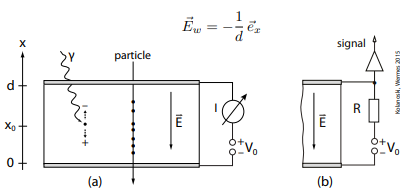
\includegraphics[width=0.7\textwidth,frame]{Chapters/images/Interazione_radiazione_materia/image-20220223210231074.png}
\end{figure}
Il campo è $E=-\frac{V}{d} \;\hat{x}$ quindi il campo di weighting è $E_w=-\frac{1}{d}\hat{x}$ e quindi la corrente generata da elettroni e ioni è

\[
    \begin{gathered}
        i_s^\pm=-\frac{q^\pm}{d}\vec{v}_D^\pm \; \hat{x}
        \\ 
        T^-=\frac{d-x_0}{{v}_D^-} \; ; \; T^+=\frac{x_0}{{v}_D^+}
    \end{gathered}
\]
dove $T^\pm$ sono le durate dei due segnali (ovvero il tempo che le cariche ci mettono ad arrivare agli elettrodi)


\begin{minipage}{0.48\textwidth}
    \vspace{-2pt}
    \begin{figure}[H]
        \centering
        \captionsetup{width=\textwidth}
        \caption{Segnale della corrente misurata agli elettrodi.\\ In questo caso il rapporto tra le velocità di drift è posto a 1/3 ma tipicamente è 1/1000}
        \vspace{-7pt}
        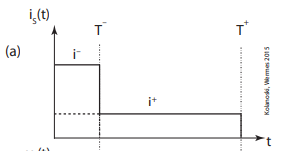
\includegraphics[width=\textwidth,frame]{Chapters/images/Interazione_radiazione_materia/image-20220223211327802.png}

        \label{fig:}
    \end{figure}
    \vspace{-30pt}
    \begin{figure}[H]
        \centering
        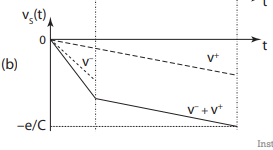
\includegraphics[width=\textwidth,frame]{Chapters/images/Interazione_radiazione_materia/image-20220223212101007.png}
        \captionsetup{width=\textwidth}
        \vspace{-23pt}
        \caption{Si può anche misurare il voltaggio invece della corrente.\\ 
        Per farlo basta inserire in una resistenza con la ionization chamber che fa da condensatore. Il tempo RC  del circuito deve essere maggiore del tempo di drift}
        \label{fig:}
    \end{figure}
\end{minipage} \hfill
\begin{minipage}{0.48\textwidth}
    \vspace{3pt}
    \begin{figure}[H]
        \centering
        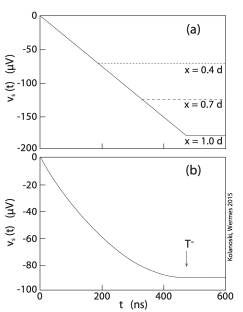
\includegraphics[width=\textwidth,frame]{Chapters/images/Interazione_radiazione_materia/image-20220223212235264.png}
        \captionsetup{width=\textwidth}
        \vspace{-19pt}
        \caption{Se invece di avere una signola carica prodotta abbiamo una linea lungo il quale vengono prodotte le cariche (traccia della particella) bisogna sommare i diversi contributi\\ A: Voltaggi misurati per singola carica prodotta\\ B: Somma dei contributi per una line di cariche}
        \label{fig:}
    \end{figure}

\end{minipage}
\sssec{Contatori proporzionali}
\begin{figure}[H]
    \centering
    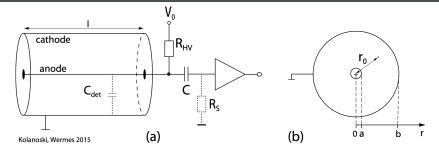
\includegraphics[width=0.7\textwidth,frame]{Chapters/images/Interazione_radiazione_materia/image-20220223212504142.png}

\end{figure}
In simmetria cilindrica il campo di weighting è $\vec{E}_w=\frac{1}{r}\frac{1}{\ln(b/a)} \; \hat{r}$ dove b e a dono il raggio di anodo e catodo
\\ 
Dalla dipendenza $1/r$ ne consegue che il segnale è dominato dal modo vicino all'anodo.
Vicino all'anodo avviene moltiplicazione di carica per un fattore $10^3-10^6$. 
\\ 
Questo significa che il segnale è dominato dal moto degli ioni prodotti dalla moltiplicazione che attraversano tutta la distanza che va dall'anodo al catodo
\begin{figure}[H]
    \centering
    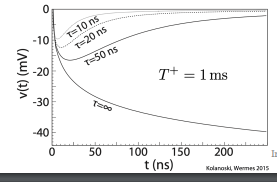
\includegraphics[width=0.5\textwidth,frame]{Chapters/images/Interazione_radiazione_materia/image-20220223213221551.png}
    \captionsetup{width=0.5\textwidth}
    \caption{La forma del segnale è principalmene stabilita dal circuito di lettura e del suo tempo caratteristico}
\end{figure}

\sssec{Detector a semiconduttore}

\begin{figure}[H]
    \centering
    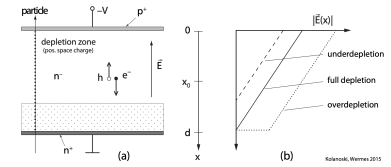
\includegraphics[width=0.7\textwidth,frame]{Chapters/images/Interazione_radiazione_materia/image-20220223213733948.png}
    \captionsetup{width=0.9\textwidth}
    \caption{Nei semiconduttori il campo elettrico non è costante a causa della presenza di molte cariche spaziali (soprattutto nella depleted zone)}
\end{figure}

\begin{figure}[H]
    \centering
    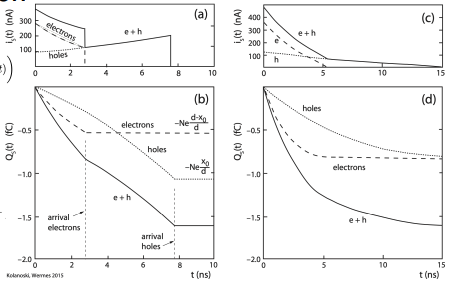
\includegraphics[width=0.7\textwidth,frame]{Chapters/images/Interazione_radiazione_materia/image-20220223213850670.png}
    \captionsetup{width=0.7\textwidth}
    \captionsetup{width=0.9\textwidth}
    \caption{Quindi in questo caso la forma dei segnali è molto più complicata ma sono essenzialmente sezioni di esponenziale (poichè il campo elettrico è lineare in funzione della posizione nella depletion zone)}
    \label{fig:}
\end{figure}

\begin{remark}[Elettrodi segmentati] \hfill \\ 
    Quando si hanno elettrodi segmentati (es. delle strip) anche se la carica verrà collezionata da un elettrodo anche gli altri vicini vedranno un segnale a causa del moto della carica
    \begin{figure}[H]
        \centering
        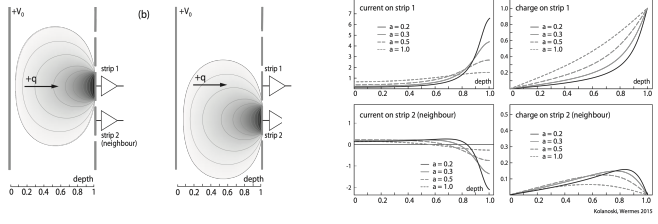
\includegraphics[width=0.7\textwidth,frame]{Chapters/images/Interazione_radiazione_materia/image-20220223214312686.png}
    \end{figure}
    Sulla strip 2 la corrente è negativa perchè vicino alla strip il campo di weighting cambia segno
\end{remark}

\section{Rumore}\footnote{Questa parte (sul rumore) l'ho tirata via molto a caso. Se vuoi qualcosa di più preciso vai a riprendere gli appunti sull'analisi dati delle onde gravitazionali}
\begin{figure}[H]
    \centering
    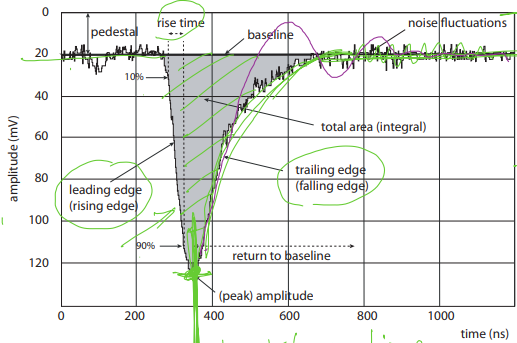
\includegraphics[width=0.7\textwidth,frame]{Chapters/images/Interazione_radiazione_materia/image-20220223230311045.png}
    \captionsetup{width=0.7\textwidth}
    \caption{Tipico segnale osservato in uscita di un detector.\\ Il tempo di rise dipende principalmente dalle caratteristiche del rivelatore ma quello di rilassamento principalmente dall'elettronica.\\ Volendo si può studiare anche la carica accumulata considerando l'area del segnale}
\end{figure}

\begin{definition*}
    \textbf{undershoot}: Quando si hanno segnali molto veloci in risalit il segnale può avere un picco che va sopra lo 0. 
In questo caso non si può usare l'area del segnale per studiare la carica collezionata

\end{definition*}

\begin{figure}[H]
    \centering
    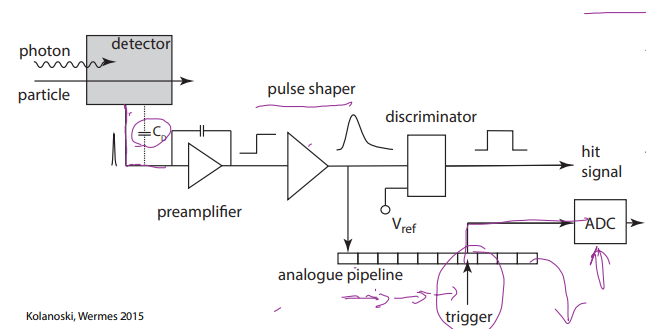
\includegraphics[width=0.7\textwidth,frame]{Chapters/images/Interazione_radiazione_materia/image-20220223230709058.png}
    \captionsetup{width=0.7\textwidth}
    \caption{Tipica catena di lettura}
\end{figure}
Per lo studio del rumore facciamo un \textbf{assunzione di ergodicità} ovvero che $<g(x)>=lim_{T\to \infty} \int_0^T g(x(t))dt$. In questo modo possiamo usare le misure fatte su $x(t)$

Alcune quantità e relazioni importanti sono:
\begin{itemize}
    \item \textbf{Autocorrelazione}  $\phi(\tau)=\overline{X(t)X(t+\tau)}$:
    \begin{itemize}
        \item E' indipendente da t poichè consideriamo il processo stazionario
        \item $\phi(0)=Var(X)$
        \item Se $\phi(\tau)\propto \delta(\tau)$ siamo in presenza di \textbf{rumore bianco}
    \end{itemize}
    \item \textbf{Densità spettrale} $S_x(f)=lim_{T\to \infty}2T\; \overline{a_na_n^*}|_{n=fT}$ dove gli $a_n $ sono i coefficienti della serie di Fourier.
    \begin{itemize}
        \item Questa quantità è legata alla varianza del segnale per unità di frequenza. Più precisamente vale $S_x(f)df=\overline{x_n^2}$ (che è la varianza se segnale  stazionario a media nulla)

\item Legata alla funzione di autocorrelazione tramite una trasformata di Fourier

\item Dimensioni: $V^2/Hz$ oppure $A^2/Hz$

\item Spesso si usa la sua radice (ovvero la amplitude spectral density)

\item Dato un segnale in input X, una funzione di trasferimento g(f) e un segnale di output Y vale:
  $S_Y(f)=|g(f)|^2 S_X(f)$ .

  Per misurare $S_X$ in genere si usa un amplificatore molto piccato intorno una frequenza $f_0$ e s i usa approssimazione $$\begin{gathered}
      \overline{Y^2}=\int_0^\infty |g(f)|^2 S_X(f)df\sim S_X(f_0)|g(f_0)|^2\int_0^\infty |\frac{g(f)}{g(f_0)}|^2  \implies \\  \implies S_X(f_0)=\frac{\overline{Y^2}}{g(f_0)^2B_N}
  \end{gathered}$$ dove $B_N$ è l'ultimo integrale rimanente sopra e viene chiamato \textit{gain bandwidth product}
    \end{itemize}
\end{itemize}

\subsection{Sorgenti di rumore}
\begin{itemize}
    \item \textbf{Rumore termico (Jhonson)}: Dovuto all'agitazione termica delle cariche ai capi di una resistenza

    E' un rumore bianco con PSD $S_V(f)=4kTR$ dove R è la resistenza (o se misuriamo la corrente $S_I=4kT/R$ poichè $I^2=V^2/R^2$)
  
  \item \textbf{Shot noise}: fluttuazione poissoniana del numero di portatori di carica $S_I=2\overline{I}e$
    (La dim. si effettua semplicemente facendo il calcolo della PSD partendo da un segnale $\overline{I(t)}=\sum_i e\delta(t-t_i)$)
  
   \begin{note}
    sia il rumore termico che lo shot noise sono rumore bianco
   \end{note} 
  
  \item \textbf{Rumore 1/f}: Rumore non ancora ben compreso dovuto a fenomeni di interfaccia. Empiricamente ha PSD $S_V=A/f^\alpha$ con $\alpha \sim 0.8-1.5$ e A costante
  
  \item Le varie PDS dovute ai diversi tipi di rumore vanno somate in quadratura
  
  Le sorgenti di rumore possono essere:
  
  \item \textbf{Detector}: a causa di rumori termici, correnti di age e fenomeni induttivi e autoinduttivi
  \item \textbf{Elettronica}: Rumore intrinsico dei componenti attivi, capacità in input (compreso il detector), altri fenomeni induttivi e autoinduttivi
  \item \textbf{Trasmissione}: Resistenza, capacità e induttanza/autoinduttanza dei cavi
  
  E' molto importante mantenere alto il \textbf{rapporto segnale rumore (SNR)}.
  Il rumore effettivo del sistema dipende dalle proprietà di filtraggio dell'amplificatore e la capacità in input gioca un ruolo fondamentale (grandi capacità causano rumori maggiori).
  
  Per tenere sotto controllo rumore termico e quello shot bisogna mantenere correnti basse, temperature basse e bandwidth strette.
  Il rumore 1/f invece dipende dal processo di fabbricaazione.
  
  Anche la massa gioca un ruolo fondamentale, tutte le masse devono finire nello stesso identico pozzo
\end{itemize}

\begin{eg}[Misuramento di carica] \hfill \\ 
    In un sistema simile si vuole massimizzare il rapporto segnale rumore inteso come carica/deviazione standard del segnale (detto anche ENC)
Considerando tutti gli errori e sommandoli in quadratura 

\begin{figure}[H]
    \centering
    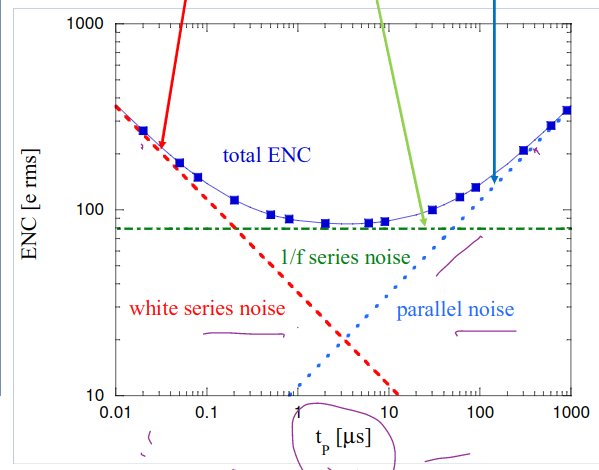
\includegraphics[width=0.7\textwidth,frame]{Chapters/images/Interazione_radiazione_materia/image-20220302174553973.png}
    \captionsetup{width=0.7\textwidth}
    \caption{$t_p$ è il tempo di picco ovvero il tempo necessario a raggiungere il picco del segnale)}

\end{figure}
si nota come bisogna scegliere un tradeoff tra diverse situazioni
\end{eg}
\chapter{Particle Identification}
\section{Radiazione Cherenkov}
L'effetto Cherenkov si ha quando una particella attraversa un mezzo con velocità superiore a quella della luce nel mezzo stesso ($c_n=c_0/n$).
\\ \\ 
La radiazione Cherenkov è causata dalla polarizzazione asimmetrica del mezzo al passaggio della particella che, rilassandosi e tornando all'equilibrio, genera una radiazione di dipolo (questo succede per ogni sezione infinitesima della traccia della particella)

\begin{figure}[H]
    \centering
    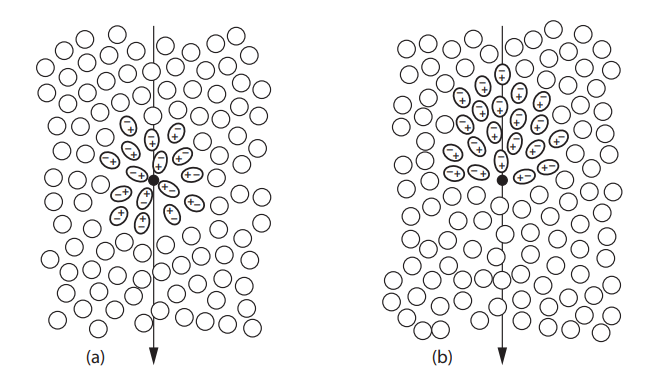
\includegraphics[width=0.7\textwidth,frame]{Chapters/images/Particle_identification/image-20220316192558631.png}
    \captionsetup{width=0.7\textwidth}
    \caption{A: Una particella a bassa velocità polarizza il mezzo in modo simmetrico\\ \\ B: A velocità superiori a quella della luce nel mezzo la polarizzazione diventa fortemente asimmetrica}
    \label{fig:}
\end{figure}

\hspace{-20pt}
\begin{minipage}{0.6\textwidth}
    \begin{figure}[H]
        \centering
        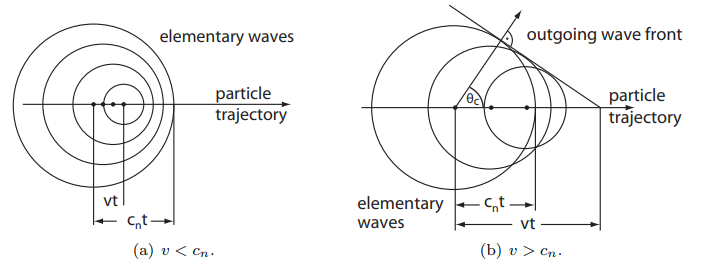
\includegraphics[width=\textwidth,frame]{Chapters/images/Particle_identification/image-20220316193152123.png}
        \captionsetup{width=\textwidth}
        \caption{Da questa figura si può ricavare facilmente l'angolo Cherenkov}
        \label{fig:}
    \end{figure}
\end{minipage} \hspace{5pt}
\begin{minipage}{0.35\textwidth}

    Ogni punto della traccia genera un'onda e se la particella ha $v>c_n$ (con $c_n$ velocità di fase della luce nel mezzo) queste onde interferiscono in modo costruttivo

\end{minipage}
L'emissione Cherenkov avviene ad un angolo fissato che aumenta con la velocità della particella
\[\cos(\theta_C)=\frac{1}{\beta n}\]
\begin{note}[Rinculo]
    Il rinculo causato dall'emissione del fotone è trascurata ma calcoli in QM mostrano che questa approssimazione è valida nella maggior parte dei casi

\end{note}
Questo angolo se misurato può subire uno \textbf{smearing}  dovuto alla relazione di dispersione del mezzo che non è costante nella frequenza

\begin{tcolorbox}[colback=NavyBlue!5]
\textbf{Recap}: La radiazione Cherenkov avviene se:
\begin{itemize}
    \item La particella ha velocità maggiore alla velocità di fase nel mezzo alla data frequenza di emissione (poichè per relazione di dispersione $n=n(\omega)$)
\item Il mezzo è trasparente nell'ottico e ha dimensioni superiori alla linghezza d'onda della radiazione (necessario per permettere l'interferenza costruttiva)

\end{itemize}

Inoltre, a una distanza sufficiente dalla traccia della particella, le onde hanno polarizzazione trasversa: sono polarizzate linearmente in un piano contenente la direzione di propagazione dell'onda e la traccia della particella
\end{tcolorbox}

\subsection{Cherenkov Threshold}
La \textbf{velocità minima}  per cui si ha emissione Cherenkov si ottiene ponendo $\cos(\theta_C)=1$ (Ovvero emissione in avanti a $0°$)
\[\beta_\text{th}=\frac{1}{n}\]
All'aumentare di $\beta$ cresce sia l'angolo che l'intensità dell'emissione.\\ 
L'\textbf{angolo massimo}  invece si ottiene per $\beta=1$
\[\begin{gathered}
    \cos(\theta_\text{max})=\frac{1}{n}
\\ 
\sin\theta_\text{max}=\sqrt{1-\cos(\theta_\text{max})^2}=\sqrt{1-\frac{1}{n^2}}=\frac{1}{\gamma_\text{th}}
\end{gathered}\]

\hspace{-10pt}
\begin{minipage}{0.6\textwidth}
    
    \begin{figure}[H]
        \centering
        \includegraphics[width=1.01\textwidth,frame]{Chapters/images/Particle_identification/image-20220317114142322.png}
    \end{figure}
\end{minipage} \hspace{5pt}
\begin{minipage}{0.41\textwidth}
\vspace{9pt}
    \begin{figure}[H]
        \captionsetup{width=\textwidth}
        \caption{Facendo il plot dell'angolo cherenkov normalizzato in funzione del $\gamma$ (normalizzato) si nota come il range di sensibilità di un rivelatore cherenkov è molto stretto dato che oltre una certa velocità la variazione dell'angolo di emissione è quasi nulla.\\ Già a $\gamma=2 \gamma_\text{th}$ l'angolo cherenkov ha raggiunto l'87\% del suo valore asintotico $\theta_\text{max}$}
    \end{figure}


\end{minipage}
Con semplici conti è possibile esprimere il seno dell'angolo in funzione di gamma
\[\begin{gathered}
    \sin^2(\theta_C)=\sin^2(\theta_\text{max})\frac{\gamma^2-\gamma_\text{th}^2}{\gamma^2-1} \implies
\\ 
\implies \lim_{\gamma \to \infty} \frac{\theta_c}{\theta_\text{max}} \simeq \frac{R_c}{R_\text{max}} \simeq \sqrt{1-\frac{\gamma_\text{th}^2}{\gamma^2}}
\end{gathered}\]
dove $R_c$ ed $R_\text{max}$ sono i raggi dei rispettivi anelli cherenkov.

\subsection{Spettro di emissione}
\begin{theorem*}[Formula di Frank-Tamm] \hfill \\ 
    Si ha radiazione Cherenkov solo per $\beta ^{2} n^{2} (\omega )>1$ e lo spettro è:
    \[\frac{d^{2}  E}{ d\omega  \: dx}  = \frac{z^{2} e^{2} }{4\pi \epsilon _{0} c^{2} }\omega \mathexplain[cd]{\left( 1-\frac{1}{\beta ^{2} n^{2}(\omega ) } \right)}{\sin ^{2} \theta _{c} (\omega )}  \]
\end{theorem*}

\begin{remark} \hfill \\
    \vspace{-20pt}
    \begin{itemize}
        \item \textbf{Si noti la linearità nella frequenza} 
        \item Le perdite di energia per luce Cherenkov sono già inluse nella Bethe Bloch ma sono largamente trascurabili: costituiscono meno dell'1\% della perdita di energia nei materiali pesanti e possono arrivare al massimo al 5\% nei gas leggeri
    \end{itemize}


\end{remark}
Un semplice modello per la permittività del mezzo è dato dalla semplice somma sulle sue frequenze di risonanza trascuranto i termini di smorzamento
\[\epsilon(\omega)=1+\frac{n_ae^2}{\epsilon_0m_e}\sum_i \frac{f_i}{\omega_{0i}^2-\omega^2}\]
con $n_a$ densità degli atomi e $f_i$ ampiezza relativa alla frequenza di risonanza i-esima con normalizzazione $\sum_i f_i=Z$.
\begin{note} 
    Ovviamente trattando gli elettroni come oscillatori senza smorzamento si ottiene una divergenza non fisica

\end{note}



\hspace{-15pt}
\begin{minipage}{0.48\textwidth}
    \begin{figure}[H]
        \centering
        \includegraphics[width=\textwidth,frame]{Chapters/images/Particle_identification/image-20220317143923078.png}
        \captionsetup{width=\textwidth}
        \caption{Poichè l'emissione avviene solo per $n^2>\frac{1}{\beta^2}$ da plot di questo tipo possiamo individuare le bande di frequenze $\Delta \omega_i$ in cui avviene l'emissione}
    \end{figure}
\end{minipage} \hspace{5pt}
\begin{minipage}{0.48\textwidth}

    Inoltre, per materiali non magnetici ($\mu \sim 1$) vale $n(\omega)\sim\sqrt{\epsilon(\omega)}$\\ 
(In realtà $\epsilon$ ha anche una parte immaginaria che causa assorbimento)
\begin{details}["Fun" fact]\hfill \\
    Il fatto che nelle vasche di raffreddamento delle centrali nucleari si veda luce blu è dovuto sia al fatto che lo spettro Cherenkov è più spostato sul blu, sia al fatto che per scattering raylight la luce a frequenza maggiore viene diffusa maggiormente, sia all'assorbimento della luce a più bassa frequenza, sia alla curva di risposta dell'occhio umani

\end{details}
    

\end{minipage}

\begin{figure}[H]
    \centering
    \includegraphics[width=0.95\textwidth,frame]{Chapters/images/Particle_identification/image-20220317154755537.png}
    \captionsetup{width=0.95\textwidth}
    \caption{Le linee tratteggiate rappresentano le zone di dispersione anomala\\ Per un mezzo reale trasparente nell'ottico sono presenti anche:\\-  zone a $n<1$ in cui non si può avere emissione. \\- Bande di emissione nell'infrarosso e nel radio (e anche a energie quasi discrete nella regione degli X)}
    \label{fig:}
\end{figure}

\sssec{Spettro dei singoli fotoni}
Dividendo la formula di Frank Tamm per l'energia di un singolo fotone $E=\hbar \omega$ si ottiene
\[\frac{d^2N}{dEdx}= \frac{\alpha}{\hbar c}z^2\left( 1-\frac{1}{\beta^2n^2(\omega)} \right) \xrightarrow{z=1} \; \sim 370 \sin^2(\theta_C)/eV/cm\]
con $\alpha=e^2/(4\pi \epsilon_0 \hbar c)$
\begin{note} questa equazione non ha nulla di quantistico, è stato inserito un $\hbar$ solo perchè si è scelto di raggruppare tutte le costanti con la costante di struttura fine

\end{note}
Usando la relazione $\omega=2\pi c / \lambda$ otteniamo
\[
\frac{d^2N}{d\lambda dx}=\frac{2\pi z^2 \alpha}{\lambda^2}\sin^2(\theta_c(\lambda))\]

\begin{remark}\hfill \\
    Quindi lo spettro $\frac{dN}{d\omega}=Const.$ mentre $\frac{dN}{d\lambda}\propto\frac{1}{\lambda^2}$
\end{remark}
Integrando su $x$, data L la lunghezza del mezzo, si ha
\[\frac{dN}{d\lambda}=\frac{2\pi z^2 \alpha}{\lambda^2}L\sin^2(\theta_c(\lambda)) \xrightarrow{\lambda \to \infty}\frac{2\pi z^2 \alpha}{\lambda^2}\frac{L}{\gamma_\text{th}^2}
\]
\hspace{-5pt}
\begin{minipage}{0.65\textwidth}
    \begin{figure}[H]
        \centering
        \includegraphics[width=\textwidth,frame]{Chapters/images/Particle_identification/image-20220317171549887.png}

    \end{figure}
\end{minipage} \hspace{5pt}
\begin{minipage}{0.35\textwidth}
\begin{figure}[H]
    \centering
    \captionsetup{width=\textwidth}
    \caption{Dipendenza dalla lunghezza d'onda dello spettro cherenkov. \\ Nell'UV c'è un cutoff dovuto alla dispersione anomala del mezzo}
\end{figure}
    

\end{minipage}

\sssec{Photon Yield}
Per ottenere il numero di fotoni ottici emessi integriamo lo spettro nella regione ottica.
Assumendo $n$ (e quindi $\theta_c$) costante nella regione ottica abbiamo
\[N_\text{opt}=z^2L\sin^2(\theta_c)\int_{400nm}^{700nm}\frac{2\pi \alpha}{\lambda^2}d\lambda\simeq z^2L\sin^2(\theta_c) \cdot \left(491 \frac{\text{ photons}}{cm}\right)\]

Quindi, soprattutto nel caso di indici di rifrazione molto bassi, il numero di fotoni può essere molto basso (spesso ci si ritrova a dover ricostruire anelli con 10 fotoni)
\\ 
Il numero di \textbf{fotoelettroni}  dipende anche da T($\lambda$): trasmittanza della finestra del dector, Q($\lambda$): efficienza quantica, R($\lambda$): riflettività degli specchi usati per focalizzare i fotoni sul detector
\[N_{pe}=2 \pi \alpha z^2 L \sin^2(\theta_c)\int_{\lambda_{1}}^{\lambda_{2}}T(\lambda)\: Q(\lambda) \: R(\lambda) \: \frac{1}{\lambda^2}d\lambda\]
\begin{details}\hfill \\
    \textit{L'integrale è chiamato figure of merit e caratterizza totalmente la risposta del detector } \\ 
    Valori tipici per il prodotto delle 3 funzioni di risposta sono intorno al 30\% ($Q\sim0.4$ , $T\sim0.8$,  $R\sim1$) quindi solitamente $N_{pe}\sim L \sin^2(\theta_c) \cdot150 (\text{photons}/cm)$
\end{details}
Anche qui è possibile normalizzare il numero di fotoni rispetto il caso asintotico (effettuando l'appossimazione $\sin(\theta_c)\sim \theta_c$)
\[\frac{N_\gamma}{N_\infty}\sim\frac{\theta_c^2}{\theta^2_\text{max}}\sim1-\frac{\gamma^2_\text{th}}{\gamma^2}\]

\begin{figure}[H]
    \centering
    \includegraphics[width=0.7\textwidth,frame]{Chapters/images/Particle_identification/image-20220317174427644.png}
    \captionsetup{width=0.7\textwidth}
    \caption{Numero di fotoelettroni in funzione di $\gamma$ per diversi materiali con $L=20cm$ e $ Q \cdot T \cdot R \sim 0.35$}
    \label{fig:}
\end{figure}

\subsection{Tipi di detector Cherenkov}
L'effetto cherenkov può essere sfruttato in diversi modi:
\begin{itemize}
    \item Threshold: seleziona solo particelle al di sopra di una certa velocità
\item Time of Flight
\item Particle identification
\item Misura di $\beta$ (e se impulso noto da altri detector anche massa)
\end{itemize}

\sssec{Threshold}



\begin{minipage}{0.4\textwidth}
    \begin{figure}[H]
        \centering
        \includegraphics[width=\textwidth,frame]{Chapters/images/Particle_identification/image-20220317181632663.png}

    \end{figure}
\end{minipage} \hspace{10pt}
\begin{minipage}{0.55\textwidth}

    In questi detector non viene misurato l'angolo Cherenkov e si ha solo una risposta si/no.\\ 
    L'impulso di soglia è $p_\text{th}=mc^2(\beta \gamma)_\text{th}=\frac{mc^2}{\sqrt{n^2-1}}$
Se il momento è noto da altri detector (spesso sfruttando un cambo magnetico) si  può usare il detector cherenkov come soglia sulla massa $m_{th}c^2=p\sqrt{n^2-1}$

\begin{details}
    
    Spesso come mezzo viene usato un gas in quanto è possibile modificare $n$, e quindi la soglia, al variare della pressione del gas

\end{details}
\end{minipage}
Se vogliamo osservare un range di energia troppo grande conviene usare più detector in successione con threshold crescente in modo tale che i detector si "accendono" in sequenza e misurando l'impulso è possibile fare \textbf{PID} 

\begin{figure}[H]
    \centering
    \includegraphics[width=0.8\textwidth,frame]{Chapters/images/Particle_identification/image-20220317185548344.png}
    \captionsetup{width=0.8\textwidth}
    \caption{Particle identification con 3 detector Cherenkov a threshold}
    \label{fig:}
\end{figure}

\begin{note}
    $\theta_c$ non viene misurato nei threshold counter

\end{note}
\vspace{-10pt}
\paragraph*{Risoluzione di un threshold detector}
Volendo si può fare particle identification con questi detector misurando il numero di fotoni emessi.
\\ 
L'incertezza legata al numero di fotoni è
 $\sigma_N=\frac{\partial N}{\partial \theta_c}\sigma_{\theta_c}=\frac{2N}{\tan(\theta_c)}\sigma_{\theta_c}= \sqrt{N}$ dove $\sigma(\theta_c)$ è lo spread angolare che varia con $\beta$
 \begin{details}
    \begin{itemize}
        \item Dopo quella derivata si è moltiplicato e diviso per $\sin(\theta_c)$ per riscrivere il numero di fotoelettroni e la tangente
        \item $\sigma_N=\sqrt{N}$ poichè statistica sui conteggi è poissoniana

    \end{itemize}
 
 \end{details}
 La risoluzione su $\beta$ invece è  (usando $\beta=1/(n \cos(\theta_c))$)
$\sigma_\beta=\frac{\partial \beta}{\partial \theta_c} \; \sigma_{\theta_c}=\beta \tan(\theta_c)$
\\ 
Quindi mettendo tutto insieme si tronva $\frac{\sigma_\beta}{\beta}=\frac{\tan^2(\theta_c)}{1\sqrt{N}}$

\sssec{RICH (Ring Imaging Cherenkov Detector)}

%─────Appendix────────────────────────────────────────────────────────────────────────────────────────────────────────────────────────────────────────

\appendix
\appendixpage
\iffalse


\fi
\chapter{Info utili}

\begin{figure}[H]
    \centering
    \includegraphics[width=0.8\textwidth]{./Chapters/images/Appendice/image-20220214164823650.png}
    \caption{Unità di misure usate in fisica delle alte energie}
    \label{fig:}
\end{figure}

% TODO Aggiungi massa particelle più importanti

% TODO Aggiungi dati su materiali più importanti

% TODO Aggiungi info utili da pdg man mano che fai esercizi

\begin{itemize}
    \item Sorgenti radioattive più usate: \url{https://pdg.lbl.gov/2018/reviews/rpp2018-rev-commonly-used-radioactive-sources.pdf}
    \item Proprietà di alcuni elementi, Stopping power e range per muoni  e lunghezze di assorbimento adroniche per pioni : \url{https://pdg.lbl.gov/2020/AtomicNuclearProperties/index.html} 
    \item NIST stopping powers for electrons and positrons in arbitrary materials: \url{http://physics.nist.gov/PhysRefData/Star/Text/ESTAR.html}
    \item NIST stopping power and range tables for protons in selected materials: \url{http://physics.nist.gov/PhysRefData/Star/Text/PSTAR.html}
    \item NIST stopping power and range tables for alpha particles in selected materials: \url{physics.nist.gov/PhysRefData/Star/Text/ASTAR.html}
\end{itemize}


\newpage
%─────Reference──────────────────────────────────────────────────────────────────────────────────────────────────────────────────────────────────────
\printbibliography

\end{document}